%% LyX 2.3.6.2 created this file.  For more info, see http://www.lyx.org/.
%% Do not edit unless you really know what you are doing.
\documentclass[twocolumn,conference]{IEEEtran}
\usepackage[T1]{fontenc}
\usepackage[latin9]{inputenc}
\usepackage{color}
\usepackage{verbatim}
\usepackage{booktabs}
\usepackage{textcomp}
\usepackage{url}
\usepackage{amsmath}
\usepackage{amssymb}
\usepackage{stmaryrd}
\usepackage{graphicx}
\usepackage{setspace}
\usepackage[unicode=true,
 bookmarks=true,bookmarksnumbered=true,bookmarksopen=true,bookmarksopenlevel=1,
 breaklinks=false,pdfborder={0 0 0},pdfborderstyle={},backref=false,colorlinks=false]
 {hyperref}
\hypersetup{pdftitle={Your Title},
 pdfauthor={Your Name},
 pdfpagelayout=OneColumn, pdfnewwindow=true, pdfstartview=XYZ, plainpages=false}

\makeatletter

%%%%%%%%%%%%%%%%%%%%%%%%%%%%%% LyX specific LaTeX commands.
%% Because html converters don't know tabularnewline
\providecommand{\tabularnewline}{\\}

%%%%%%%%%%%%%%%%%%%%%%%%%%%%%% Textclass specific LaTeX commands.
\newenvironment{lyxcode}
	{\par\begin{list}{}{
		\setlength{\rightmargin}{\leftmargin}
		\setlength{\listparindent}{0pt}% needed for AMS classes
		\raggedright
		\setlength{\itemsep}{0pt}
		\setlength{\parsep}{0pt}
		\normalfont\ttfamily}%
	 \item[]}
	{\end{list}}

%%%%%%%%%%%%%%%%%%%%%%%%%%%%%% User specified LaTeX commands.
% for subfigures/subtables
\usepackage[caption=false,font=footnotesize]{subfig}
\usepackage{hyperref}
\hypersetup{colorlinks=true}
\usepackage[dvipsnames]{xcolor}
\definecolor{lgray}{rgb}{0.95, 0.95, 0.95}
\usepackage{mathtools}

\@ifundefined{showcaptionsetup}{}{%
 \PassOptionsToPackage{caption=false}{subfig}}
\usepackage{subfig}
\makeatother

\usepackage{minted}
\renewcommand{\listingscaption}{Listing}

\begin{document}
\title{\texttt{BraggHLS}}
\author{\IEEEauthorblockN{Maksim~Levental}\IEEEauthorblockA{University of Chicago\\
Email: test@test.tes}\and \IEEEauthorblockN{Ryan~Chard}\IEEEauthorblockA{Ecole Superieure\\
Nantes, France\\
Email: second@second.fr}\and \IEEEauthorblockN{Kyle~Chard\\
and Ian~Foster}\IEEEauthorblockA{Star Academy\\
San Francisco, California 99999-9999\\
Telephone: (800) 555\textendash 5555\\
Fax: (888) 555\textendash 5555}}
\maketitle
\begin{abstract}
In many experiment-driven scientific domains, such as high-energy
physics, material science, and cosmology, very high data rate experiments
impose hard constraints on the corresponding data acquisition systems:
collected data must either be indiscriminately stored for post-processing
and analysis, thereby necessitating large storage capacity, or accurately
filtered in real-time, thereby necessitating low latency execution.
Deep neural networks, effective in many other filtering tasks, have
not been widely employed in such data acquisition systems, due to
design and deployment difficulties. This paper presents an open source,
lightweight, compiler framework \texttt{BraggHLS}, based on high-level
synthesis techniques, for translating high-level representations of
deep neural networks to low-level representations, suitable for deployment
to near-sensor devices such as field-programmable gate arrays. We
evaluate \texttt{BraggHLS} on various workloads and present a case-study
implementation of a deep neural network for Bragg peak detection in
the context of high-energy diffraction microscopy. We show \texttt{BraggHLS}
is able to produce an implementation of the network with a throughput
4.8 \textmu s/sample, which is approximately a 4$\times$ improvement
over the existing implementation.

\tableofcontents{}
\end{abstract}


\section{Introduction\label{sec:Introduction}}

Very high data rates are observed and, consequently, large datasets
are generated across a broad range of experiments in scientific domains,
such as high-energy physics, material science, and cosmology. For
example, in high-energy physics, the LHCb detector, at the CERN Large
Hadron Collider, is tasked with observing the trajectories of particles
produced in proton-proton collisions at a rate of 40 million per second
(i.e., 40 MHz) \cite{pmlr-v42-glig14}. With a packet size of approximately
50 kB (per collision), this implies a data rate of approximately 2
TB/s. Ultimately, in combination with other detectors, the LHC processes
approximately 100 EB of data a year. In materials science, high-energy
diffraction microscopy (HEDM) techniques, which provide non-destructive
characterization of structure and its evolution in a broad class of
single-crystal and polycrystalline materials, can have collection
rates approaching 1 MHz \cite{Hammer_2021}, with a corresponding
packet size of 80 kB. In cosmology, the Square Kilometer Array, a
radio telescope projected to be completed in 2024 and to be operational
by 2027 \cite{mcmullin2022square}, will sustain data rates in excess
of 10 TB/s \cite{grainge2017square}.

Naturally, for high data rate experiments, directly storing and distributing
such large quantities of data to the associated research communities
for further analysis is cost prohibitive. Thus, either compression
(in the case of storage and transmission) or outright filtering is
necessary, i.e., only a small fraction of the most ``interesting''
data is selected at time of collection, with the remainder being permanently
discarded. In this work we focus on the filtering approach. Note,
the tradeoff made in employing filtering should be clear: reduced
storage at the expense of more stringent latency constraints (on the
filtering mechanisms). In addition, the risk of discarding meaningful
data introduces accuracy (of the filtering mechanisms) as a critical
new dimension of the data acquisition systems. Typically, these filtering
mechanisms consist either of physics based models \cite{LHCB-FIGURE-2020-018}
or machine learning models \cite{Gligorov_2013}; in either case maximally
efficient and effective use of the target hardware platform is tantamount
to accuracy. Irrespective of the type of technique employed, almost
universally, for the ultra-low latency use cases (e.g., sub-microsecond
latency constraints), the implementation is deployed to either field-programmable
gate arrays (FPGAs) or application-specific integrated circuits (ASICs)
\cite{Duarte_2018}. Here we focus primarily on FPGAs.%
\begin{comment}
The reason for this is only FPGAs and ASICs are flexible enough to
satisfy the latency constraints for a wide range of techniques. Note,
in this work we focus exclusively on FPGAs.
\end{comment}

Deep neural networks (DNNs), a particular type of machine learning
model, have been shown to be effective in many scientific and commercial
domains due to their ``representational capacity'', i.e., they demonstrate
a capacity to (approximately) represent diverse sets of mappings \cite{alzubaidi2021review}.
DNNs ``learn'' to represent a mapping over the course of ``training'',
wherein they are iteratively evaluated on sample data while a ``learning
rule'' periodically updates the parameters (\emph{weights}) that
parameterize the DNN. In recent years they have been investigated
for near real-time scientific use cases \cite{liu2019deep,patton2018167,liu2022exploring}
but their use for the lowest latency use cases has been very limited
\cite{Duarte_2018}. The reasons for this are threefold: 
\begin{enumerate}
\item Graphics Processing Units (GPUs), the conventional hardware target
for DNNs, until very recently, have not been performant enough for
these very high data rate, very low latency, use cases (due to their
low clock speeds and low peripheral bandwidth \cite{aaij2020allen});
\item DNNs, by virtue of their depth, are resource intensive, in terms of
both memory (for the weights) and compute (floating-point arithmetic),
thereby preventing their deployment to FPGAs, which, in particular,
have limited static RAM available;
\item DNNs are (typically) defined, trained, and distributed using high-level
frameworks (such as PyTorch \cite{paszke2017automatic}, TensorFlow
\cite{https://doi.org/10.48550/arxiv.1603.04467}, MXNet \cite{https://doi.org/10.48550/arxiv.1512.01274}),
which abstract all implementation details from the user, thereby making
portability of existing model architectures (to e.g., FPGA) nigh impossible.
\end{enumerate}
These three barriers demand of a solution that can simultaneously
translate a high-level representation of a DNN to a low-level representation,
suitable for deployment to FPGA, while optimizing resource usage and
minimizing latency. In general, the task of \emph{lowering} high-level
representations of programs to lower-level representations is the
domain of a compiler. Similarly, the task of \emph{synthesizing} a\emph{
register-transfer level} (RTL) \emph{design}, rendered in a \emph{hardware
description language} (HDL), from a program, is the domain of high-level
synthesis (HLS) \cite{7368920}. While several such HLS tools exist
\cite{10.1145/2514740,Zhang2008,ferrandi2021bambu} and despite, often,
bundling robust optimizing compilers, they struggle to effectively
perform the necessary optimizations in reasonable amounts of time
(see Section \ref{subsec:High-level-synthesis}).

Recently, deep learning compilers (such as TVM \cite{chen2018tvm},
MLIR \cite{https://doi.org/10.48550/arxiv.2002.11054}, and Glow \cite{https://doi.org/10.48550/arxiv.1805.00907})
have demonstrated the ability to dramatically reduce inference latencies
\cite{https://doi.org/10.48550/arxiv.1809.02697}, training times
\cite{9664259}, and memory usage \cite{https://doi.org/10.48550/arxiv.1604.06174}
of DNNs. These compilers function by extracting intermediate-level
representations (IRs) of the DNNs, from the representations produced
by the frameworks, and performing various optimizations on those IRs
(such as kernel fusion \cite{10.1145/2858788.2688521}, vectorization
\cite{maleki2011evaluation}, and memory planning \cite{https://doi.org/10.48550/arxiv.1604.06174}).
The highly optimized IR is then used to generate code for various
target hardware platforms. Given the successes of these compilers,
it's natural to wonder whether they can adapted to the task of sufficiently
optimizing a DNN such that it might be synthesized to RTL, for deployment
to FPGA.

In this paper, we present \texttt{BraggHLS}, an open source, lightweight,
compiler and HLS framework which can lower DNNs defined as PyTorch
models to FPGA compatible implementations. \texttt{BraggHLS} uses
a combination of compiler and HLS techniques to compile the entire
DNN into fully scheduled RTL, thereby eliminating all synchronization
overheads and achieving ultra-low latency. \texttt{BraggHLS} is general
and supports a wide range of DNN layer types, and thus a wide range
of DNNs, but we particularly focus on optimizations relevant to a
DNN designed for identifying Bragg diffraction peaks. In summary our
specific contributions include:
\begin{enumerate}
\item We describe and implement a compiler framework, \texttt{BraggHLS},
which can effectively transform unoptimized, hardware-agnostic PyTorch
models into ultra-low latency RTL designs suitable for deployment
to Xilinx FPGAs. \texttt{BraggHLS} is thoroughly tested, open source,
and available at \href{https://github.com/makslevental/bragghls/}{https://github.com/makslevental/bragghls/};
\item We show that designs generated by \texttt{BraggHLS} achieve lower
latency than Xilinx's state-of-the-art commercial HLS tool (Vitis
HLS) for a variety of DNN layer types. In particular we show that
\texttt{BraggHLS} can produce synthesizable designs that meet placement,
routing, and timing constraints for \texttt{BraggNN}, a DNN designed
for identifying Bragg diffraction peaks;
\item We discuss some of the challanges faced even after successful synthesis
of RTL from a high-level representation of a DNN, namely during the
place and route phases of implementation.
\end{enumerate}
The rest of this paper is organized as follows: Section \ref{sec:Background}
reviews key concepts from compilers, high-level synthesis, and RTL
design for FPGA. Section \ref{sec:BraggHLS-compiler-and} describes
the \texttt{BraggHLS} compiler and HLS framework in detail. Section
\ref{sec:Evaluation} evaluates \texttt{BraggHLS}\textquoteright s
performance, scalability, and competitiveness with designs generated
by Vitis HLS. Section \ref{sec:BraggNN-case-study} describes our
case study, i.e., \texttt{BraggHLS} applied to \texttt{BraggNN}, a
Bragg peak detection DNN with a target latency of 1 \textmu s/sample.
Finally, Section \ref{sec:Conclusion} concludes with a summary, and
related and future work.

\section{Background\label{sec:Background}}

\subsection{Compilers: the path from high to low}

The path from a high-level, abstract, representation of a DNN to a
register-transfer level representation can be neatly formulated as
a series of progressive lowerings between adjacent levels of abstraction.
Each level of abstraction is rendered as a programming language, IR,
or HDL, and thus we describe each lowering in terms the representations
and tools \texttt{BraggHLS} employ in manipulating those representations:
\begin{enumerate}
\item An imperative, \emph{define-by-run,} Python representation, in PyTorch;
\item High-level data-flow graph representation, in TorchScript;
\item Low-level data and control flow graph representation, in MLIR.
\end{enumerate}
%

\subsubsection{PyTorch and TorchScript}

Typically DNN models are represented in terms high-level frameworks,
themselves implemented within general purpose programming languages.
Such frameworks are widely used because of their ease of use and large
library of example implementations of various DNN model architectures.
\texttt{BraggHLS} is targets the PyTorch framework, thus we focus
on relevant aspects of PyTorch. DNNs developed within PyTorch are
\emph{defined-by-run}: the author imperatively describes the DNN in
terms of high-level operations, using python, which when executed
materializes the (partial) high-level data-flow graph (DFG) corresponding
to the DNN (e.g., for the purposes of reverse-mode automatic differentiation).
From the perspective of the user, define-by-run enables fast iteration
at development time, possibly at the cost of some runtime performance. 

On the other hand, from the perspective of compilation, define-by-run
precludes efficient extraction of the high-level DFG; since the DFG
is materialized only at runtime, it cannot be inferred from the textual
representation (i.e., the python source) of the DNN. Furthermore,
a priori, the runtime-materialized DFG is only partially materialized\footnote{``...instead, every intermediate result records only the subset of
the computation graph that was relevant to their computation.'' \cite{paszke2017automatic}}, and only as an in-memory data structure. Thus, framework support
is necessary for efficiently extracting the full DFG. Indeed, PyTorch
supports a Single Static Assignment (SSA) IR, called TorchScript (TS)
IR and accompanying tracing mechanism (the TS JIT), which produces
TS IR from conventionally defined PyTorch models. Lowering from PyTorch
to TS IR enables various useful analyses and transformations on a
DNN at the level of the high-level DFG (such as kernel fusion \cite{10.1145/2858788.2688521})
but targeting FPGAs requires a broader collection of transformations.
To this end, we turn to a recent addition to the compiler ecosystem.

\subsubsection{MLIR\label{subsec:MLIR}}

Multi-level Intermediate Representation \cite{https://doi.org/10.48550/arxiv.2002.11054}
presents a new approach to building reusable and extensible compiler
infrastructure. MLIR is composed of a set of \emph{dialect} IRs, subsets
of which are mutually compatible, either outright or by way of translation/legalization.
The various dialects aim to capture and formalize the semantics of
compute intensive programs at varying levels of abstraction, as well
as namespace related sets of IR transformations. The entrypoint into
this compiler framework, from PyTorch, is the \texttt{torch} dialect
\cite{torch-mlir}, a high-fidelity mapping from TS IR to MLIR native
IR, which, in addition to performing the translation to MLIR, fully
refines all shapes of intermediate tensors in the DNN (i.e., computes
concrete values for all dimensions of each tensor); this is necessary
for downstream optimizations and eliminating inconsistencies in the
DNN \cite{https://doi.org/10.48550/arxiv.2203.08402}.

While the \texttt{torch} dialect is necessary for lowering to MLIR
and shape refinement, it is a representation of a DNN at the same
level of abstraction as TS IR: it does not capture the precise data
flow and control flow necessary for de novo implementations of DNN
operations (e.g., for FPGA). Fortunately, MLIR supports lower-level
dialects, such as the \texttt{linalg}, \texttt{affine} and \texttt{scf}
(structured control flow) dialects. The \texttt{scf} dialect describes
standard control flow primitives, such as conditionals and loops,
and is mutually compatible with the \texttt{arith} (arithmetic operations)
and \texttt{memref} (memory buffers) dialects. The \texttt{affine}
dialect, on the other hand, provides a formalization of semantics
that lend themselves to polyhedral compilation techniques \cite{polyhedral-mlir},
i.e., techniques that enable loop dependence analysis and loop transformations.
Such loop transformations, particularly loop unrolling, are crucial
for achieving lowest possible latencies \cite{yehpca2022scalehls}
because they directly inform the concurrency and parallelism of the
final RTL design.

\subsection{High-level synthesis and FPGA design}

\subsubsection{High-level synthesis\label{subsec:High-level-synthesis}}

High-level synthesis tools produce RTL descriptions of designs from
high-level representations, such as C or C++ \cite{10.1145/2514740,ferrandi2021bambu}.
In particular, Xilinx's Vitis HLS, based on the Autopilot project
\cite{Zhang2008}, is a state-of-the-art HLS tool. Given a high-level,
procedural, representation, HLS carries out three fundamental tasks,
in order to produce a corresponding RTL design:
\begin{enumerate}
\item HLS schedules operations (such as \texttt{mulf}, \texttt{addf}, \texttt{load},
\texttt{store}) in order to determine which operations should occur
during each clock cycle; such a schedule depends on three characteristics
of the high-level representation:
\begin{enumerate}
\item The topological ordering of the DFG/CFG of the procedural representation
(i.e., the dependencies of operations on results of other operations
and resources);
\item The completion time for each operation;
\item The user's desired clock rate/frequency;
\end{enumerate}
\item HLS associates (called \emph{binding}) operations to particular RTL
instantiations of intellectual property (IP) for those operations;
for example whether to associate an addition operation followed by
a multiply operation to IPs for each, or whether to associate them
both with a single IP, designed to perform a ``fused'' multiply-accumulate
(MAC);
\begin{enumerate}
\item In the case of floating-point arithmetic operations, HLS also (with
user guidance) determines the precision of the floating-point representation;
\end{enumerate}
\item HLS builds a finite-state machine (FSM) that implements the schedule
of operations as control logic, i.e., logic that initiates operations
during the appropriate stages of the schedule.
\end{enumerate}
In addition to fulfilling these three fundamental tasks, high-level
synthesis aims to optimize the program. In particular, HLS attempts
to maximize concurrency and parallelism (number of concurrent operations
scheduled during a clock-cycle) in order maximize the throughput and
minimize the latency of the final implementation. Maximizing concurrency
entails pipelining operations: operations are executed such that they
overlap in time, subject to available resources. Maximizing parallelism
entails partitioning the DNN into subsets of operation that can be
computed independently and simultaneously and whose results are combined
upon completion. 

While HLS aims to optimize various characteristics of a design, there
are challenges associated with this kind of automated optimization.
In particular, maximum concurrency and parallelism necessitates data-flow
analysis in order to identify data dependencies amongst operations,
both for scheduling and identifying potential data hazards. Such data-flow
analysis is expensive and grows (in runtime) as better performance
is pursued. This can be understood in terms of loop-nest representations
of DNN operations; for example consider a convolution as in Listing
\ref{lis:Single-filter-convolution}.
\begin{listing}
\begin{minted}[fontsize={\footnotesize},escapeinside={||},mathescape=true]{python}
def conv2d(
  input: MemRef(|$b$|, |$c_{in}$|, |$h$|, |$w$|),
  output: MemRef(|$b$|, |$c_{out}$|, |$h$|, |$w$|),
  weight: MemRef(|$c_{out}$|, |$c_{in}$|, |$k$|, |$k$|)
):
  for i1 in range(0, |$b$|):
    for i2 in range(0, |$c_{out}$|):
      for i3 in range(0, |$h$|):
        for i4 in range(0, |$w$|):
          for i5 in range(0, |$c_{in}$|):
            for i6 in range(0, |$k$|):
              for i7 in range(0, |$k$|):
                _3 = i3 + i6
                _4 = i4 + i7
                _5 = input[i1, i5, _3, _4]
                _6 = weight[i2, i5, i6, i7]
                _7 = output[i1, i2, i3, i4]
                _8 = _5 * _6
                _9 = _7 + _8
                output[i1, i2, i3, i4] = _9
\end{minted}
\caption{Python representation of a padding $\left\lfloor k/2\right\rfloor $,
stride 1, $c_{out}$ filter convolution with $k\times k$ kernel applied
to ($\ensuremath{b},\ensuremath{c_{in}},\ensuremath{h},\ensuremath{w}$)-dimensional\texttt{
input} tensor, where $b$ is the batch size, $c_{in}$ is the number
of channels, and ($h,w$) are the height and width, respectively.\label{lis:Single-filter-convolution}}
\end{listing}
 A schedule that parallelizes (some of) the arithmetic operations
for this loop nest can be computed by first unrolling the loops up
to some ``trip-count'' and then computing the topological sort of
the operations. Using this scheduling algorithm (known as \emph{list
scheduling}), the degree to which the loops are unrolled determines
how many arithmetic operations can be scheduled in parallel. The issue
is that the \texttt{store}s and \texttt{load}s on the \texttt{output}
array prevent reconstruction of explicit relationships between the
inputs and outputs of the arithmetic operations across loop iterations.
The conventional resolution to this loss of information is to perform
\emph{store-load forwarding}: pairs of \texttt{store} and \texttt{load}
operations on the same memory address are eliminated, with the operand
of the \texttt{store} forwarded to the uses of the \texttt{load} (see
Listing \ref{lis:Single-filter-convolution-1}).
\begin{listing}
\begin{minted}[numbers=left,fontsize={\footnotesize},escapeinside={||},mathescape=true,highlightlines={19,25},autogobble=true,numbersep=3pt]{python}
def conv2d(
  input: MemRef(|$b$|, |$c_{in}$|, |$h$|, |$w$|),
  output: MemRef(|$b$|, |$c_{out}$|, |$h$|, |$w$|),
  weight: MemRef(|$c_{out}$|, |$c_{in}$|, |$k$|, |$k$|)
):
  for i1 in range(0, |$b$|):
    for i2 in range(0, |$c_{out}$|):
      for i3 in range(0, |$h$|):
        for i4 in range(0, |$w$|):
	  ...
	  # e.g., i5, i6, i7 = 2, 3, ${\setlength{\fboxsep}{1pt}\colorbox{Salmon}{\texttt{4}}}$
	  _31 = i3 + i6 
	  _41 = i4 + i7 
	  _51 = input[i1, i5, _31, _41] 
	  _61 = weight[i2, i5, i6, i7] 
	  _71 = output[i1, i2, i3, i4] 
	  _81 = _51 * _61 
	  |${\setlength{ \fboxsep}{1pt} \colorbox{green}{ \texttt{\_91}}}$| = _71 + _81 
	  output[i1, i2, i3, i4] = _91 
	  # i5, i6, i7 = 2, 3, ${\setlength{\fboxsep}{1pt}\colorbox{Salmon}{\texttt{5}}}$
	  _32 = i3 + i6 
	  _42 = i4 + i7 
	  _52 = input[i1, i5, _32, _42] 
	  _62 = weight[i2, i5, i6, i7] 
	  |${\setlength{\fboxsep}{1pt}\colorbox{yellow}{\texttt{\_72}}}$| = output[i1, i2, i3, i4] 
	  _82 = _52 * _62 
	  |${\setlength{\fboxsep}{1pt}\colorbox{Cyan}{\texttt{\_92}}}$| = |${\setlength{\fboxsep}{1pt}\colorbox{yellow}{\texttt{\_72}}}$| + _82 
	  output[i1, i2, i3, i4] = _92
	  ...
\end{minted}
\caption{Store-load forwarding across successive iterations (e.g.,\texttt{
i7} $={\setlength{\fboxsep}{1pt}\colorbox{Salmon}{\texttt{4}}}, {\setlength{\fboxsep}{1pt}\colorbox{Salmon}{\texttt{5}}}$)
of the inner loop in Listing \ref{lis:Single-filter-convolution},
after unrolling. The forwarding opportunity is from the store on line
19 to the load on line 25; both can be eliminated and ${\setlength{\fboxsep}{1pt}\colorbox{green}{\texttt{\_91}}}$
can replace uses of ${\setlength{\fboxsep}{1pt}\colorbox{yellow}{\texttt{\_72}}}$,
such as in the computation of \texttt{${\setlength{\fboxsep}{1pt}\colorbox{Cyan}{\texttt{\_92}}}$}
(and potentially many others).\label{lis:Single-filter-convolution-1}}
\end{listing}
 In order for this transformation to be correct (i.e., preserve program
semantics), for each pair of candidate \texttt{store} and \texttt{load}
operations, it must be verified that there are no intervening memory
operations on the same memory address. These verifications are non-trivial
since the iteration spaces of the loops need not be regular; in general
it might involve solving a small constraint satisfaction program \cite{rajopadhye2002dependence}.
Furthermore, the number of such verifications grows polynomially in
the parameters of the convolution since the loop nest unrolls into
$b\times c_{out}\times h\times w\times c_{in}\times k^{2}$ \texttt{store}-\texttt{load}
pairs on the \texttt{output} array.

Finally, note, though greedy solutions to the scheduling problem solved
by HLS are possible, in principle scheduling is an integer linear
programming problem (ILP), instances of which are NP-hard. In summary,
HLS tools solve computationally intensive problems in order to produce
a RTL description of a high-level representation of a DNN. These phases
of the HLS process incur ``development time'' costs (i.e., runtime
of the tools) and impose practical limitations on the amount of design
space exploration (for the purpose of achieving latency goals) which
can be performed. \texttt{BraggHLS} addresses these issues by enabling
the user to employ heuristics (during both the parallelization and
scheduling phases) which, while not guaranteed to be correct, can
be \emph{behaviorally verified} (see Section \ref{subsec:AST-transformations-and}).

\subsection{FPGA design}

Broadly, at the register-transfer level of abstraction, there remain
two more steps prior to being able to actually deploy a design to
an FPGA; one of them being a final lowering, so-called logic synthesis,
and the other being place and route (P\&R). The entire process is
carried out, for example, by Xilinx's Vivado tool. 

Logic synthesis is the process of mapping RTL to actual hardware primitives
on the FPGA (so-called \emph{technology mapping}), such as lookup
tables (LUTs), block RAMs (BRAMs), flip-flops (FFs), and digital signal
processors (DSPs). Logic synthesis produces a network list (\emph{netlist})
describing the logical connectivity of various parts of the design.
Logic synthesis effectively determines the implementation of floating-point
operations in terms of DSPs; depending on user parameters and other
design features, DSP resource consumption for floating-point multiplication
and addition can differ greatly. The number of LUTs and DSPs that
a high-level representation of a DNN corresponds to is relevant to
both the performance and feasibility of that DNN when deployed to
FPGA.

After the netlist has been produced, the entire design undergoes P\&R.
The goal of P\&R is to determine which configurable logic block within
an FPGA should implement each of the units of logic required by the
digital design. P\&R algorithms need to minimize distances between
related units of functionality (in order to minimize wire delay),
balance wire density across the entire fabric of the FPGA (in order
to reduce route congestion), and maximize the clock speed of the design
(a function of both wire delay, logic complexity, and route congestion).
The final, routed design, can then be deployed to the FPGA by producing
a proprietary \emph{bitstream}, which is written to the FPGA.

\section{\texttt{BraggHLS} compiler and HLS framework\label{sec:BraggHLS-compiler-and}}

\texttt{BraggHLS} is a compiler and HLS framework which employs MLIR
for extracting loop-nest representations of DNNs. It is implemented
in python for ease of use and extensibility. Critically, and distinctly,
it handles the DNN transformations as well as scheduling, binding,
and FSM extraction; there is no dependence on any commercial HLS tools.
Figure \ref{fig:BraggHLS-framework-overview.-3} shows the architecture
of \texttt{BraggHLS} 
\begin{figure}[tbh]
\centering{}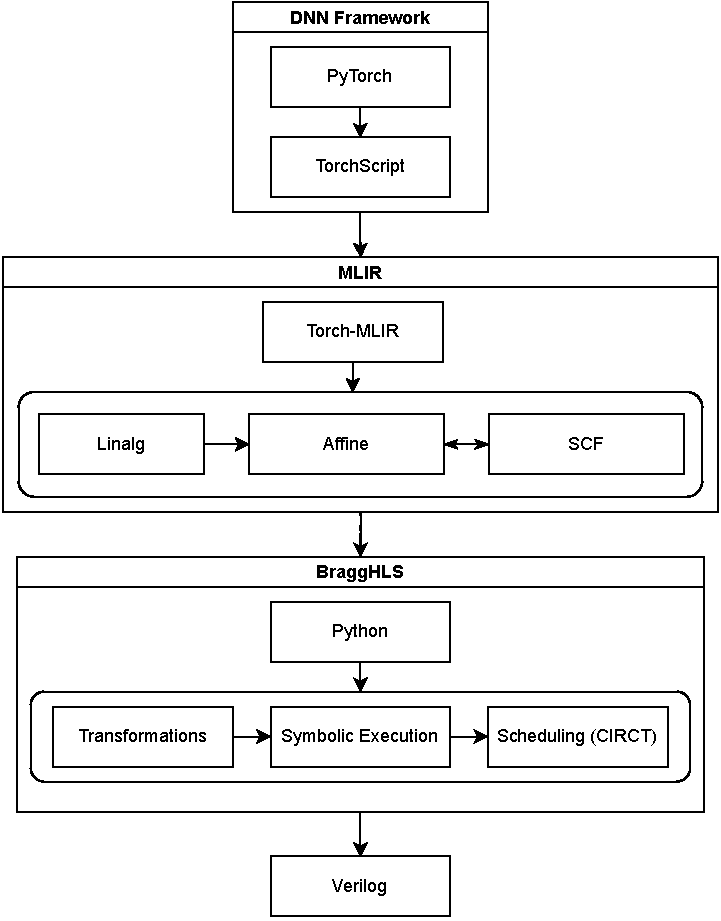
\includegraphics[width=0.7\columnwidth]{../figures/BraggHLS}\caption{\texttt{BraggHLS} framework overview (placeholder).\label{fig:BraggHLS-framework-overview.-3}}
\end{figure}
. \texttt{BraggHLS} proceeds by first lowering DNNs from PyTorch to
MLIR through TorchScript and the \texttt{torch} dialect (see Section
\ref{subsec:MLIR}). They are then further lowered from the \texttt{torch}
dialect to the \texttt{scf} dialect (through the \texttt{linalg} dialect).
Such a representation lends itself to a straightforward translation
to python (compare Listing \ref{lis:Single-filter-convolution} to
Listing \ref{lis:Single-filter-convolution}) and indeed \texttt{BraggHLS}
performs this translation.
\begin{listing}
\begin{minted}[fontsize={\footnotesize},escapeinside={||},mathescape=true]{tex}
@conv2d(
    %input: memref<|$b \times c_{in} \times h \times w$|>,
    %weight: memref<|$b \times c_{out} \times h \times w$|>,
    %output: memref<|$c_{out} \times c_{in} \times k \times k$|>
) {
  scf.for %i1 = %c0 to |$b$| step %c1 {
    scf.for %i2 = %c0 to |$c_{out}$| step %c1 {
      scf.for %i3 = %c0 to |$h$| step %c1 {
        scf.for %i4 = %c0 to |$w$| step %c1 {
          scf.for %i5 = %c0 to |$c_{in}$| step %c1 {
            scf.for %i6 = %c0 to |$k$| step %c1 {
              scf.for %i7 = %c0 to |$k$| step %c1 {
                %3 = arith.addi %i3, %i6
                %4 = arith.addi %i4, %i7
                %5 = memref.load %input[
                  %i1, %i5, %i3, %3, %4]
                %6 = memref.load %weight[
                  %i2, %i5, %i6, %i7]
                %7 = memref.load %output[
                  %i1, %i2, %i3, %i4]
                %8 = arith.mulf %5, %6
                %9 = arith.addf %7, %8
                memref.store %9, %output[
                  %i1, %i2, %i3, %i4]
              } 
            }
          }  
        }
      }
    }
  }
  return %2
}
\end{minted}
\caption{\texttt{scf} dialect loop representation of the convolution in Listing
\ref{lis:Single-filter-convolution}.\label{lis:Single-filter-convolution-2-1}}
\end{listing}
 The benefits of translating \texttt{scf} dialect to python are manifold
and discussed in the following (see Section \ref{subsec:Symbolic-execution-for}).
Ultimately, \texttt{BraggHLS} produces a representation of the DNN
that is then fully scheduled using the scheduling infrastructure in
CIRCT \cite{oppermann2022eurollvm} (an MLIR adjacent project). After
scheduling, \texttt{BraggHLS} emits corresponding RTL (as Verilog). 

\texttt{BraggHLS} delegates to the FloPoCo \cite{8877424} IP generator
the task of generating pipelined implementations of the standard floating-point
arithmetic operations (\texttt{mulf}, \texttt{divf}, \texttt{addf},
\texttt{subf}, \texttt{sqrtf}) at various precisions. In addition,
we implement a few generic (parameterized by bit width) operators
in order to support a broad range of DNN operations: two-operand maximum
(\texttt{max}); negation (\texttt{neg}); rectified linear units (\texttt{relu}).
Transcendental functions, such as \texttt{exp}, are implemented using
a Taylor series expansion to $k$-th order (where $k$ is determined
on a case-by-case basis). Note, FloPoCo's floating-point representation
differs slightly from IEEE754, foregoing subnormals and differently
encoding zeroes, infinities and NaNs (for the benefit of reduced complexity)
and our implementations \texttt{max}, \texttt{neg}, \texttt{relu}
are adjusted appropriately. 

We now discuss some aspects of \texttt{BraggHLS} in greater detail.

\subsection{Symbolic interpretation for fun and profit\label{subsec:Symbolic-execution-for}}

As discussed in Section \ref{subsec:High-level-synthesis}, maximizing
concurrency and parallelism for a design entails unrolling loop nests
and analyzing the data-flow of encompassed operations. As also discussed
in Section \ref{subsec:High-level-synthesis}, the formally correct
approach to unrolling a loop nest is prohibitively expensive in terms
of runtime. Indeed, for example, in the case of \texttt{BraggNN},
repeatedly performing this unrolling was a hindrance to effectively
searching the design space for a RTL representation achieving the
target latency, since it often took an enormous amount of time (see
Figure \ref{fig:-kernel-convolution-full}). 
\begin{figure}[tbh]
\begin{centering}
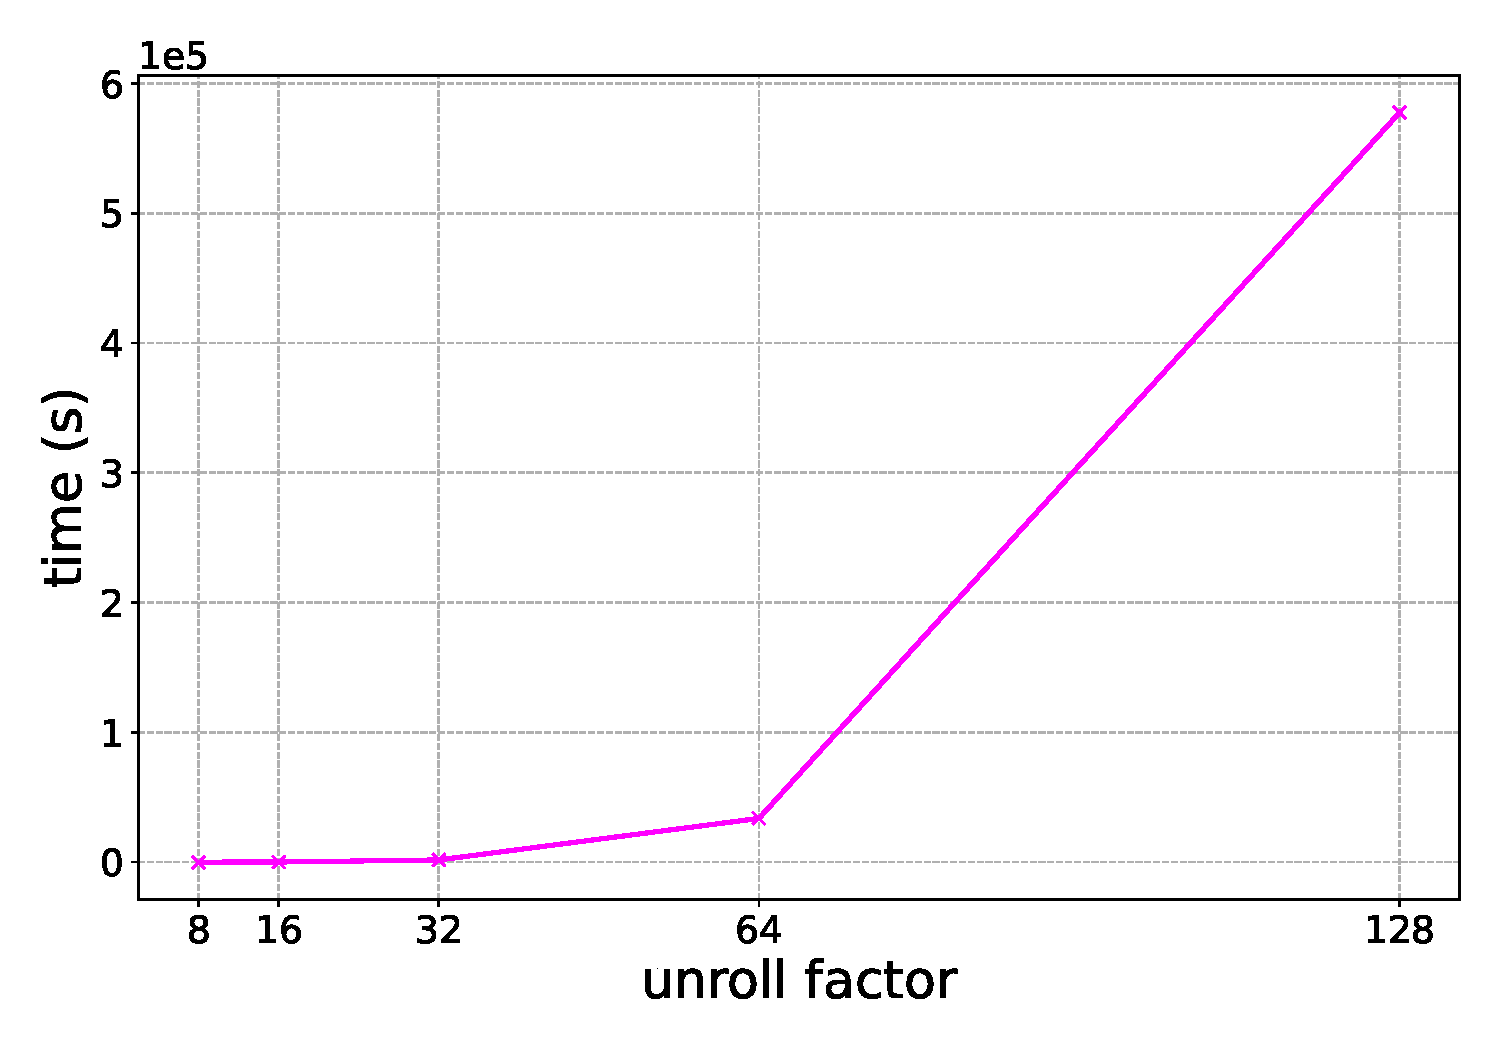
\includegraphics[width=1\columnwidth]{/Users/mlevental/dev_projects/hls_paper/data/conv_unroll}
\par\end{centering}
\caption{$3\times3$-kernel convolution full unrolling time.\label{fig:-kernel-convolution-full}}

\end{figure}
Translating \texttt{scf} dialect to python enables \texttt{BraggHLS}
to overcome this barrier by enabling us to use the python interpreter
as a \emph{symbolic interpreter}. Interpreting the resulting python
loop-nests (i.e., running the python program) while treating the arithmetic
and memory operations on SSA values as operations on symbols (i.e.,
python classes with overloaded methods) enables us to: 
\begin{enumerate}
\item Partially evaluate functions of iteration variables, such as \mintinline{mupad}!%3 = arith.addi %i3, %i6!,
which enables concretely determining array index operands of all stores
and loads, such as \mintinline[fontsize={\small}]{mupad}!memref.load %input[%i1,%i5,%i3,%3,%4]!,
and thereupon performing memory dependence checks, thus transforming
the problem of statically verifying memory dependence into a matter
of checking assertions at runtime;
\item Unroll loops by recording each floating-point arithmetic operation
executed while enforcing SSA; e.g., for a loop whose body has repeated
assignments to the same SSA value (ostensibly violating SSA), we execute
the loop and instantiate new, uniquely identified, symbols for the
result of each operation;
\item Reconstruct all data flow through arithmetic operations and memory
operations by interpreting \texttt{memref}s as \emph{geometric symbol
tables} (i.e., symbol tables indexed by array indices rather than
identifiers/names) and \texttt{store}s and \texttt{load}s as assignments
and reads on those symbol tables;
\item Easily swap evaluation rules in order to support various functionality
modes, e.g., evaluating the floating-point arithmetic operations using
(python) bindings to FloPoCo's C++ functional models thereby enabling
behavioral verification.
\end{enumerate}
See Table \ref{tab:scf-dialect-to} for the translation rules from
\texttt{\textcolor{blue}{scf}} dialect to python; with 

{\scriptsize{}}
\begin{table*}[tbh]
{\scriptsize{}\caption{\texttt{\textcolor{blue}{scf}} dialect to python translation.\label{tab:scf-dialect-to}}
}{\scriptsize\par}
\begin{doublespace}
\begin{centering}
{\small{}}%
\begin{tabular}{lll}
\toprule 
\texttt{\textcolor{blue}{\small{}scf}}{\small{} dialect} &  & {\small{}python}\tabularnewline
\midrule
{\small{}$\left\llbracket \texttt{\%5}\right\rrbracket $} &  & {\small{}$\texttt{v5 = Val("\%5")}$}\tabularnewline
{\small{}$\left\llbracket \texttt{memref<}b\times c_{in}\times h\times w\texttt{>}\right\rrbracket $} &  & {\small{}$\texttt{MemRef(\ensuremath{b}, \ensuremath{c_{in}}, \ensuremath{h}, \ensuremath{w})}$}\tabularnewline
{\small{}$\left\llbracket \texttt{\%5 = memref.load \%input[\%i1, \%i5, \%3, \%4]}\right\rrbracket $} &  & {\small{}$\texttt{\ensuremath{\left\llbracket \texttt{\%5}\right\rrbracket }= \ensuremath{\left\llbracket \texttt{\%input}\right\rrbracket }.\_\_getitem\_\_((\ensuremath{\left\llbracket \texttt{\%i1}\right\rrbracket }, \ensuremath{\left\llbracket \texttt{\%i5}\right\rrbracket }, \ensuremath{\left\llbracket \texttt{\%3}\right\rrbracket }, \ensuremath{\left\llbracket \texttt{\%4}\right\rrbracket }))}$}\tabularnewline
{\small{}$\left\llbracket \texttt{memref.store \%9, \%output[\%i1, \%i5, \%3, \%4]}\right\rrbracket $} &  & {\small{}$\texttt{\ensuremath{\left\llbracket \texttt{\%output}\right\rrbracket }.\_\_setitem\_\_((\ensuremath{\left\llbracket \texttt{\%i1}\right\rrbracket }, \ensuremath{\left\llbracket \texttt{\%i5}\right\rrbracket }, \ensuremath{\left\llbracket \texttt{\%3}\right\rrbracket }, \ensuremath{\left\llbracket \texttt{\%4}\right\rrbracket }), \ensuremath{\left\llbracket \texttt{\%9}\right\rrbracket })}$}\tabularnewline
{\small{}$\left\llbracket \texttt{scf.for \%i1 = \%c0 to }b\texttt{ step \%c1}\right\rrbracket $} &  & {\small{}$\texttt{for \ensuremath{\left\llbracket \texttt{\%iv1}\right\rrbracket }in range(\ensuremath{\left\llbracket \texttt{\%c0}\right\rrbracket }, }b\texttt{, \ensuremath{\left\llbracket \texttt{\%c1}\right\rrbracket })}$}\tabularnewline
{\small{}$\left\llbracket \texttt{\%3 = arith.addi \%i3, \%i6}\right\rrbracket $} &  & {\small{}$\texttt{\texttt{\ensuremath{\left\llbracket \texttt{\%3}\right\rrbracket }= \ensuremath{\left\llbracket \texttt{\%i3}\right\rrbracket }+ \ensuremath{\left\llbracket \texttt{\%i6}\right\rrbracket }}}$}\tabularnewline
{\small{}$\left\llbracket \texttt{\%8 = arith.mulf \%5, \%6}\right\rrbracket $} &  & {\small{}$\texttt{\texttt{\ensuremath{\left\llbracket \texttt{\%8}\right\rrbracket }= \ensuremath{\left\llbracket \texttt{\%5}\right\rrbracket }.\_\_mul\_\_(\ensuremath{\left\llbracket \texttt{\%6}\right\rrbracket }})}$}\tabularnewline
{\small{}$\left\llbracket \texttt{\%9 = arith.addf \%7, \%8}\right\rrbracket $} &  & {\small{}$\texttt{\texttt{\ensuremath{\left\llbracket \texttt{\%9}\right\rrbracket }= \ensuremath{\left\llbracket \texttt{\%7}\right\rrbracket }.\_\_add\_\_(\ensuremath{\left\llbracket \texttt{\%8}\right\rrbracket })}}$}\tabularnewline
\vspace{-15pt}
 &  & \tabularnewline
{\small{}$\left\llbracket \begin{array}{c}
\texttt{\%63 = arith.cmpfugt \%10, \%c0}\\
\texttt{\%64 = arith.select \%63, \%c0\,\,}
\end{array}\right\rrbracket $} &  & {\small{}$\texttt{\texttt{\ensuremath{\left\llbracket \texttt{\%64}\right\rrbracket }= \ensuremath{\left\llbracket \texttt{\%10}\right\rrbracket }.relu()}}$}\tabularnewline
\vspace{-10pt}
 &  & \tabularnewline
{\small{}$\left\llbracket \begin{array}{c}
\texttt{\texttt{\%8 = arith.mulf \%5, \%6}}\\
\texttt{\%9 = arith.addf \%7, \%8}
\end{array}\right\rrbracket $} &  & {\small{}$\texttt{\texttt{\ensuremath{\left\llbracket \texttt{\%9}\right\rrbracket }= fma(\ensuremath{\left\llbracket \texttt{\%5}\right\rrbracket }, \ensuremath{\left\llbracket \texttt{\%6}\right\rrbracket }, \ensuremath{\left\llbracket \texttt{\%7}\right\rrbracket })}}$}\tabularnewline
\vspace{-10pt}
 &  & \tabularnewline
\bottomrule
\end{tabular}{\small\par}
\par\end{centering}
\end{doublespace}
\begin{lyxcode}
\end{lyxcode}
\end{table*}
{\scriptsize\par}

\subsection{AST transformations and behavioral verification\label{subsec:AST-transformations-and-1}}

Prior to intepretation, \texttt{BraggHLS} performs some simple AST
transformations on the python generated from \texttt{scf} dialect:
\begin{enumerate}
\item \textbf{Hoist globals}: all DNN tensors which are fixed (i.e., weights)
are moved out of the body of the python \footnote{\texttt{BraggHLS} translates the MLIR \texttt{module} corresponding
to the DNN into a single python function in order to simplify analysis
and interpretation.} and into the parameter list, for the purpose of ultimately exposing
them at the RTL module interface; 
\item \textbf{Remove }\texttt{\textbf{if}}\textbf{ expressions}: DNN \texttt{relu}
operations are lowered to the \texttt{scf} dialect as a decomposition
of \texttt{arith.cmpfugt} and \texttt{arith.select}; this transformation
recomposes them into a \texttt{relu};
\item \textbf{Remove MACs}: sequences of \texttt{load}-\texttt{multiply}-\texttt{add}-\texttt{store}
are very common in DNN implementations, thus we schedule such sequences
jointly (this transformation coalesces such sequences into a single
\texttt{FMAC});
\item \textbf{Reduce }\texttt{\textbf{for}}\textbf{s}: this transformation
implements the reduction tree structure for non-parallelizable loop-nests
mentioned in Section \ref{subsec:Symbolic-execution-for}.
\end{enumerate}
These transformations on the python AST are simple (implemented with
procedural pattern matching), extensible, and efficient (marginal
runtime cost) because they are unverified: no effort is made to verify
their formal correctness. Thus, \texttt{BraggHLS} trades formal correctness
for development time performance. This tradeoff enables quick design
space iteration, which for example, enabled us to achieve very low
latency implementations for \texttt{BraggNN} (see Section \ref{sec:BraggNN-case-study}).
As a substitute for formal verification, \texttt{BraggHLS} supports
behavioral verification. Specifically, \texttt{BraggHLS}, can generate
testbenches for all synthesized RTL. The test vectors for these testbenches
are generated by evaluating the generated python representation of
the DNN on randomly generated inputs but with floating-point operations
now evaluated using functional models of the corresponding FloPoCo
operators. The testbenches can then be run using any IEEE 1364 compliant
simulator. For example, we run a battery of such testbenches (corresponding
to various DNN operation types), using \texttt{cocotb} \cite{rosser2018cocotb}
and \texttt{iverilog} \cite{williamsicarus}, as a part of our continuous
integration process\footnote{\url{https://github.com/makslevental/bragghls/actions}}.

\subsection{Scheduling}

Recall that one of the critical functions which HLS fulfills is the
scheduling of operations during each clock cycle, in such a way that
they preserve the data-flow graph of a DNN; that schedule then informs
the construction of a corresponding FSM. As already mentioned, scheduling
arbitrary DNNs involves formulating and solving an ILP. In the resource-unconstrained
case, due to the precedence relations induced by data-flow, the constraint
matrix of the associated ILP is \emph{totally unimodular matrix} and
the feasible region of the problem is an integral polyhedron. Thus,
in such cases, the scheduling problem can be solved optimally in polynomial
time with a LP solver \cite{tuprints9272}. In the resource-constrained
case it is possible to transform resource constraints into precedence
constraints as well, by picking a particular (possibly heuristic)
linear ordering on the particularly resource-constrained operations.
This transformation partitions resource constrained operations into
distinct clock cycles, thereby guaranteeing sufficient resources are
available for all operations scheduled within the same clock cycle
\cite{10.1145/3174243.3174268}. 

\texttt{BraggHLS} uses the explicit parallelism of the \texttt{scf.parallel}
loop-nest representation to inform such a linear ordering on resource-constrained
operations. By assumption, for loop-nests which can be reprepresented
as \texttt{scf.parallel} loop-nests (see Listing \ref{lis:Single-filter-convolution-2-2}),
each instance of a floating-point arithmetic operation in the body
corresponding to unique values of the iteration variables (e.g., \texttt{\%i1},\texttt{
\%i2},\texttt{ \%i3},\texttt{ \%i4} for Listing \ref{lis:Single-filter-convolution-2-2})
is independent of all other such instances\footnote{Data-flow within a loop body must still be respected.}.
This exactly determines total resource usage per loop-nest; for example,
the convolution in Listing \ref{lis:Single-filter-convolution-2-2},
would bind to $2K_{i}$ DSPs (assuming \texttt{mulf}, \texttt{addf}
bind to one DSP each), where
\begin{multline*}
K_{i}:=\left|\left\{ \texttt{\%iv1}=\texttt{\%c0}+\texttt{\%c1}\times\mathbb{N}\,\wedge\,\texttt{\%iv1}<b\right\} \right|\times\\
\left|\left\{ \texttt{\%iv2}=\texttt{\%c0}+\texttt{\%c1}\times\mathbb{N}\,\wedge\,\texttt{\%iv2}<c_{out}\right\} \right|\times\\
\left|\left\{ \texttt{\%iv3}=\texttt{\%c0}+\texttt{\%c1}\times\mathbb{N}\,\wedge\,\texttt{\%iv3}<h\right\} \right|\times\\
\left|\left\{ \texttt{\%iv4}=\texttt{\%c0}+\texttt{\%c1}\times\mathbb{N}\,\wedge\,\texttt{\%iv4}<w\right\} \right|
\end{multline*}
where $\texttt{\%c1}\times\mathbb{N}$ represents all multiples of
$\texttt{\%c1}$. That is to say, $K_{i}$ is the cartesian product
of the iteration spaces of the parallel iteration variables. 
\begin{listing}
\begin{minted}[fontsize={\footnotesize},escapeinside={||},mathescape=true]{mupad}
@conv2d(
    %input: memref<|$b \times c_{in} \times h \times w$|>,
    %weight: memref<|$b \times c_{out} \times h \times w$|>,
    %output: memref<|$c_{out} \times c_{in} \times k \times k$|>
) {
  scf.parallel (%i1, %i2, %i3, %i4) =
               (%c0, %c0, %c0, %c0) to
               (|$b$|, |$c_{out}$|, |$h$|, |$w$|) step
               (%c1, %c1, %c1, %c1) {
    scf.for %i5 = %c0 to |$c_{in}$| step %c1 {
      scf.for %i6 = %c0 to |$k$| step %c1 {
        scf.for %i7 = %c0 to |$k$| step %c1 {
          %3 = arith.addi %i3, %i6
          %4 = arith.addi %i4, %i7
          %5 = memref.load %input[%i1, %i5, %i3, %3, %4]
          %6 = memref.load %weight[%i2, %i5, %i6, %i7]
          %7 = memref.load %output[%i1, %i2, %i3, %i4]
          %8 = arith.mulf %5, %6
          %9 = arith.addf %7, %8
          memref.store %9, %output[%i1, %i2, %i3, %i4]
        }
      }
    }
  }
  return %2
}
\end{minted}
\caption{Parallel loop representation of the convolution in Listing \ref{lis:Single-filter-convolution}.\label{lis:Single-filter-convolution-2-2}}
\end{listing}
. Taking the maximum over such $K:=\max_{i}K_{i}$ across all \texttt{scf.parallel}
loop-nests, we can infer peak usage of any resource. Then, after indexing
available hardware resources $j=1,\dots,K$, we can bind the operations
of any particular loop-nest. This leads to a linear ordering on resource-constrained
operations such that operations bound to the same hardware resource
index $j$ must be ordered according to their execution order during
interpretation\footnote{\texttt{BraggHLS} only needs to construct a partial precedence ordering
$\texttt{op}_{a}<\texttt{op}_{b}$ for operations $\texttt{op}_{a},\texttt{op}_{b}$
which CIRCT then combines with the delays of the operations to construct
constraints such as $\texttt{start\_op}_{a}+\texttt{delay}_{a}\leq\texttt{start\_op}_{b}$.}. Note this ordering coincides with the higher-level structure of
the DNN, since ordering of\texttt{ scf.parallel} loop nests (and thus
interpretation order during execution of the python program) is determined
by the higher-level structure of the DNN.

For DNN operations that do not lower \texttt{scf.parallel} loop-nests
but lower to sequential loop nests (e.g., \texttt{sum}, \texttt{max},
or \texttt{prod}), we fully unroll the loops and transform the resulting,
sequential, operations to a reduction tree; we use As-Late-As-Possible
scheduling \cite{baruch1996scheduling} amongst the subtrees of such
reduction trees.

\section{Evaluation\label{sec:Evaluation}}

We evaluate \texttt{BraggHLS both} on individual DNN kernels (i.e.,
layers) and end-to-end, on our use-case \texttt{BraggNN}.

\subsection{DNN layers}

asdasd
\begin{figure*}[tbh]
\begin{centering}
\subfloat[\texttt{addmm}]{\centering{}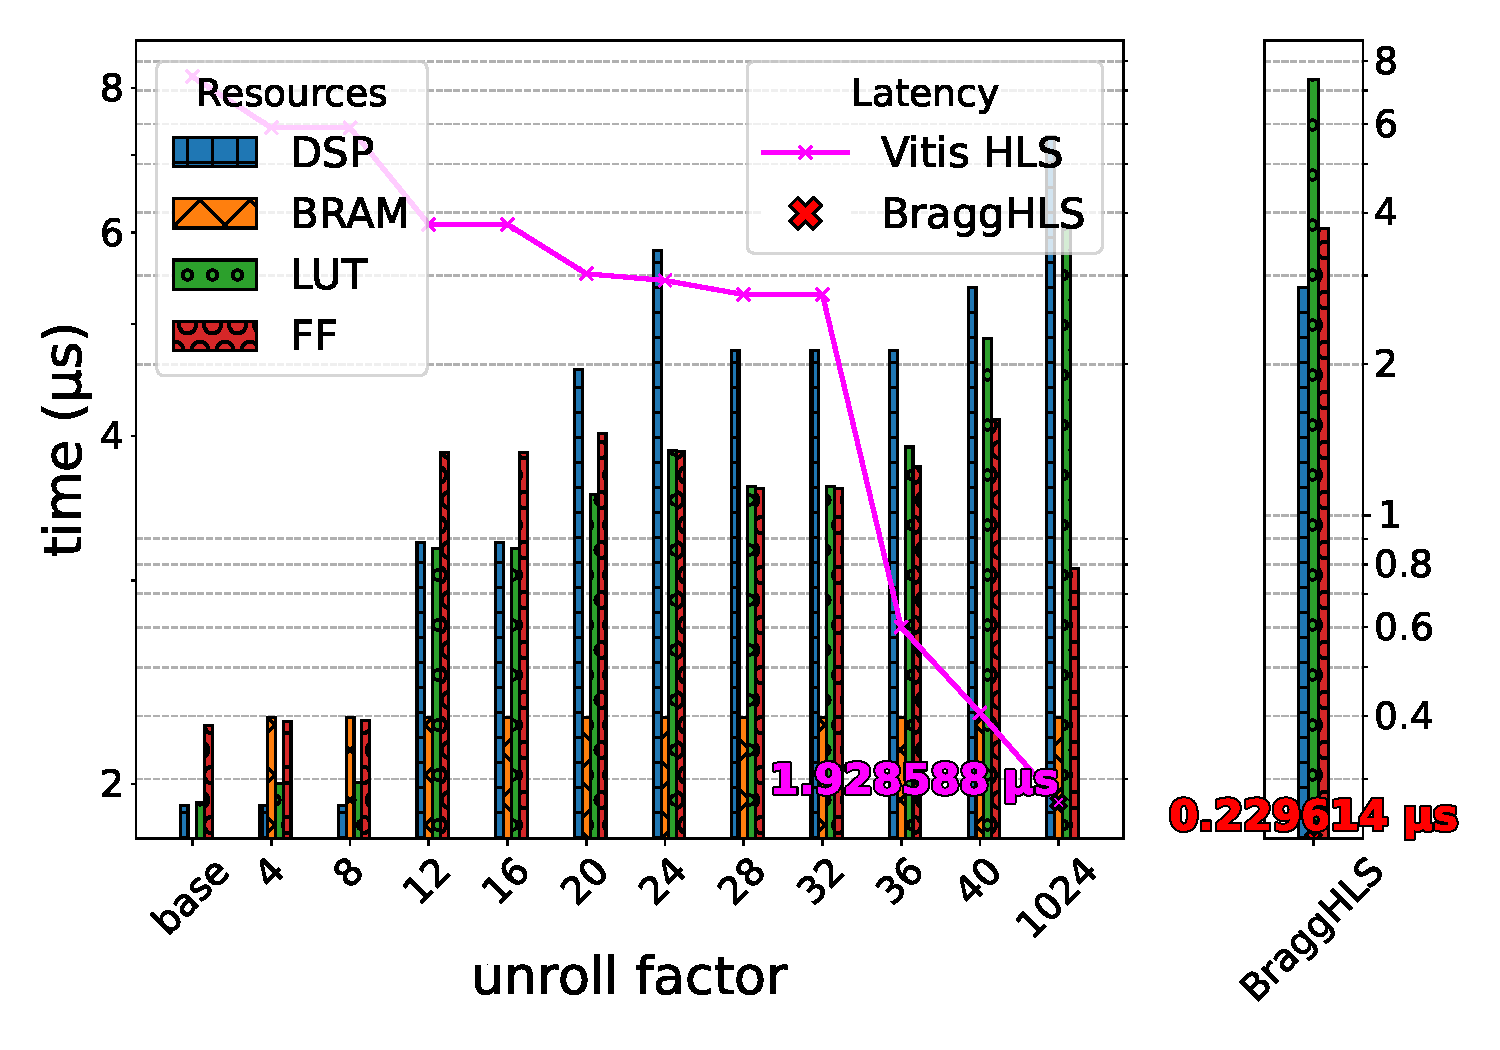
\includegraphics[width=1\columnwidth]{../figures/addmm}\label{2dlattice-1-1-2}}\subfloat[\texttt{batch\_norm}]{\centering{}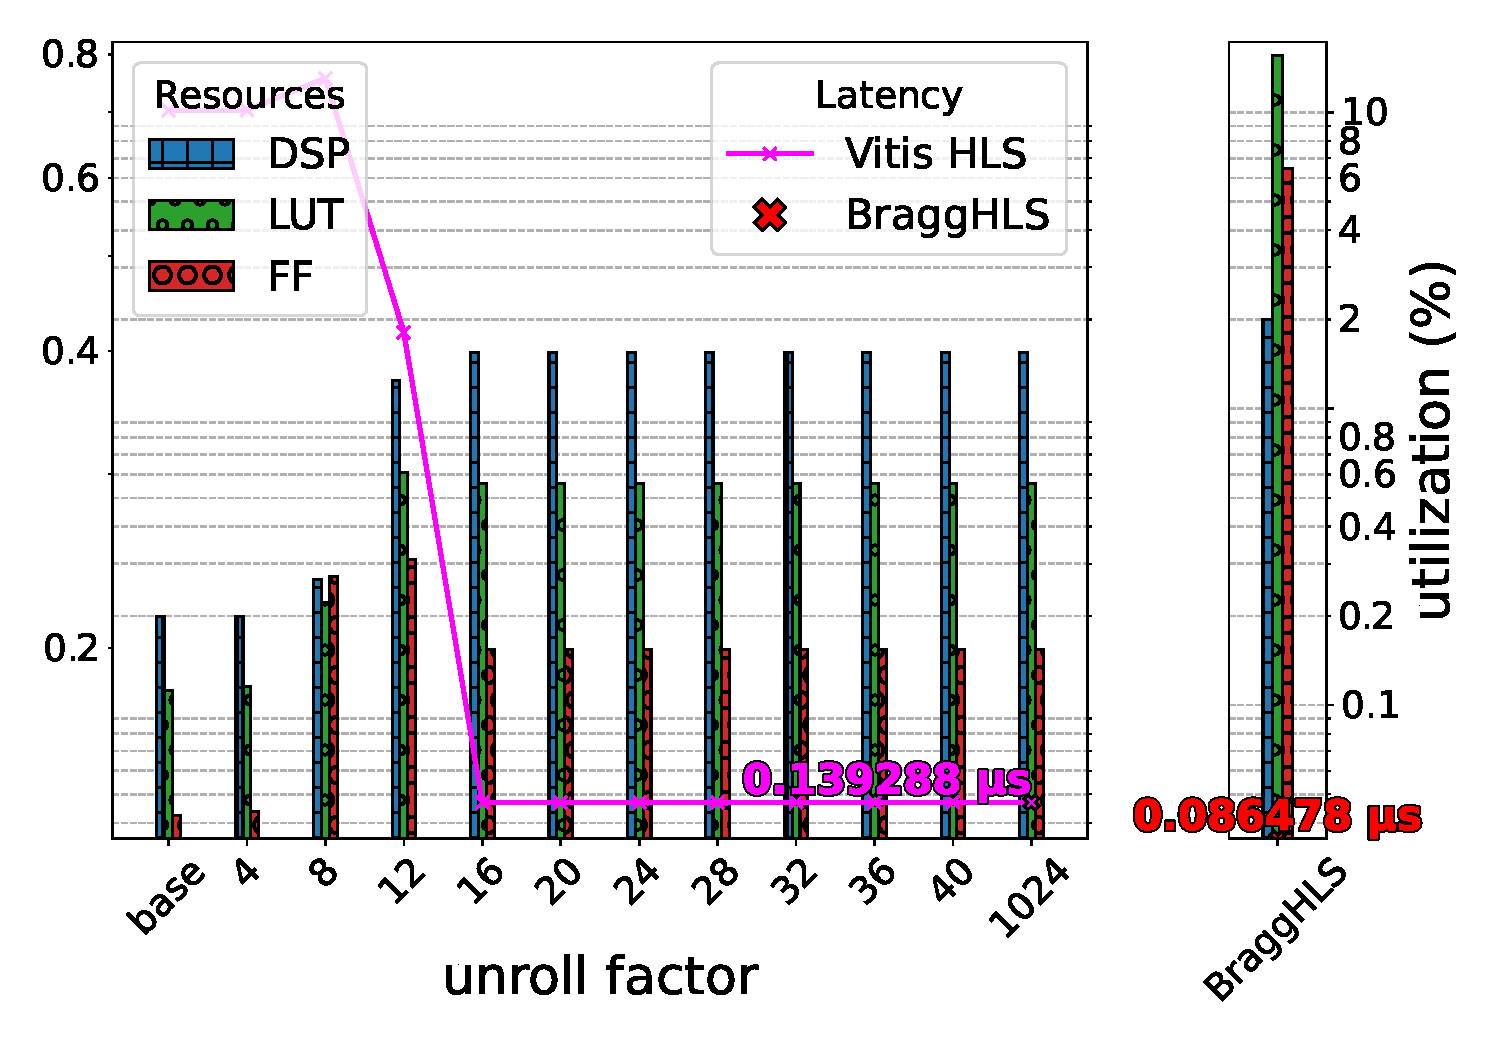
\includegraphics[width=1\columnwidth]{../figures/batch_norm}\label{2dlattice-1-2-2}}
\par\end{centering}
\medskip{}

\centering{}\label{2dlattice-1-3}\subfloat[\texttt{conv}]{\centering{}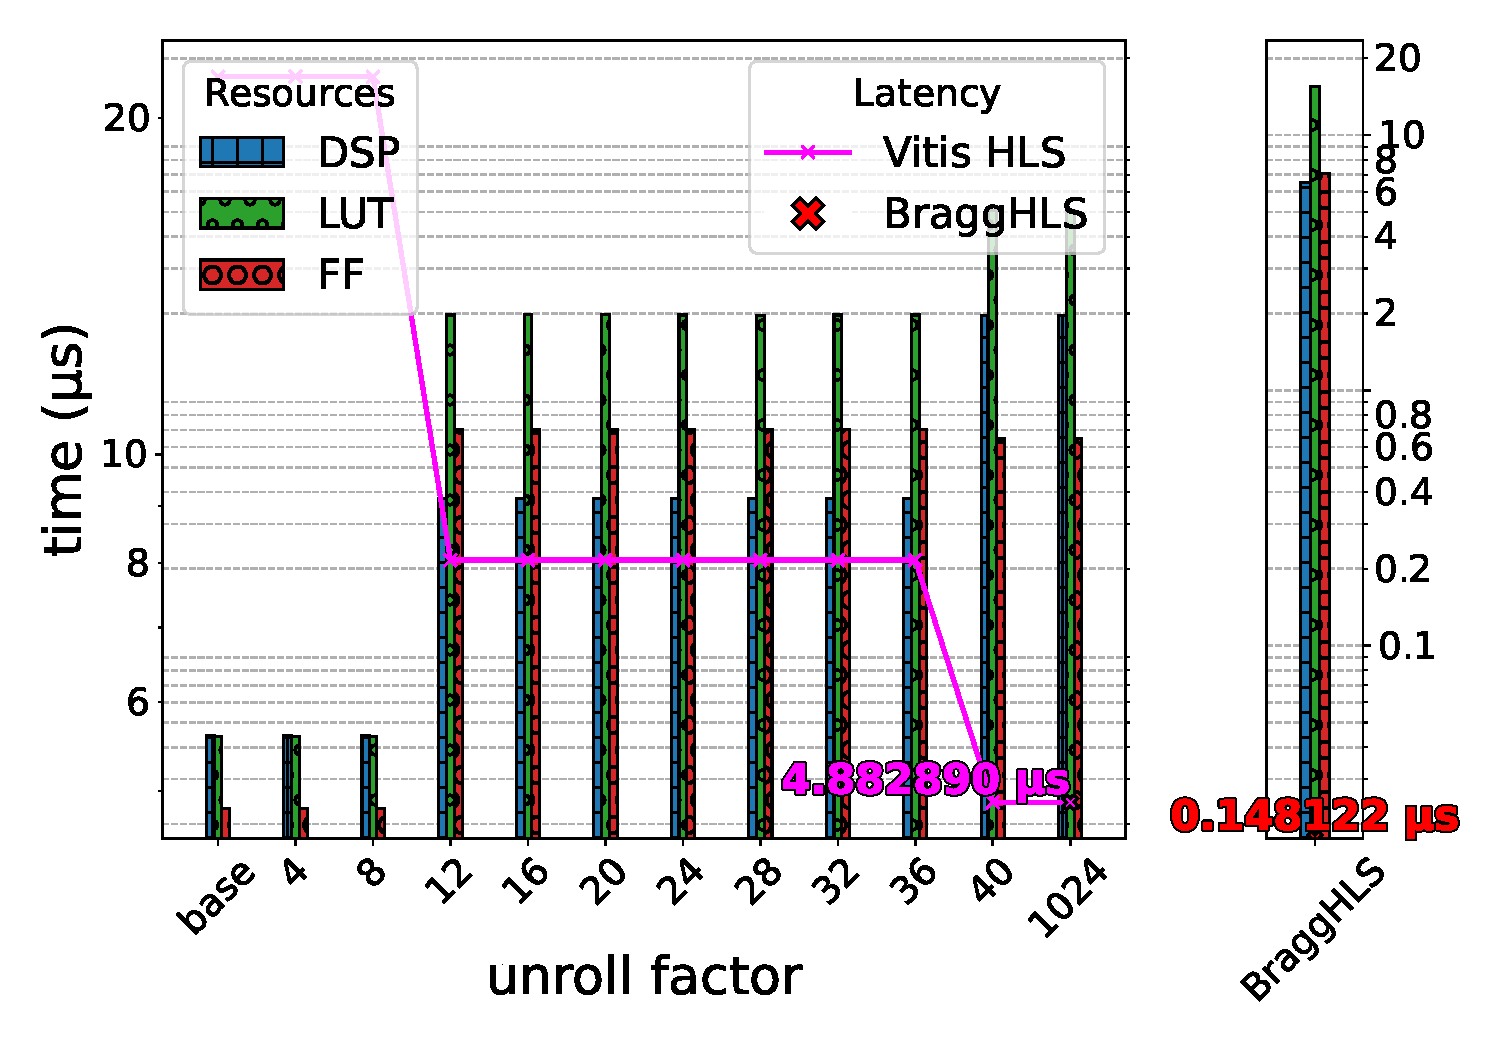
\includegraphics[width=1\columnwidth]{../figures/conv}\label{2dlattice-1-1-1-1}}\subfloat[\texttt{max\_pool\_2d}]{\centering{}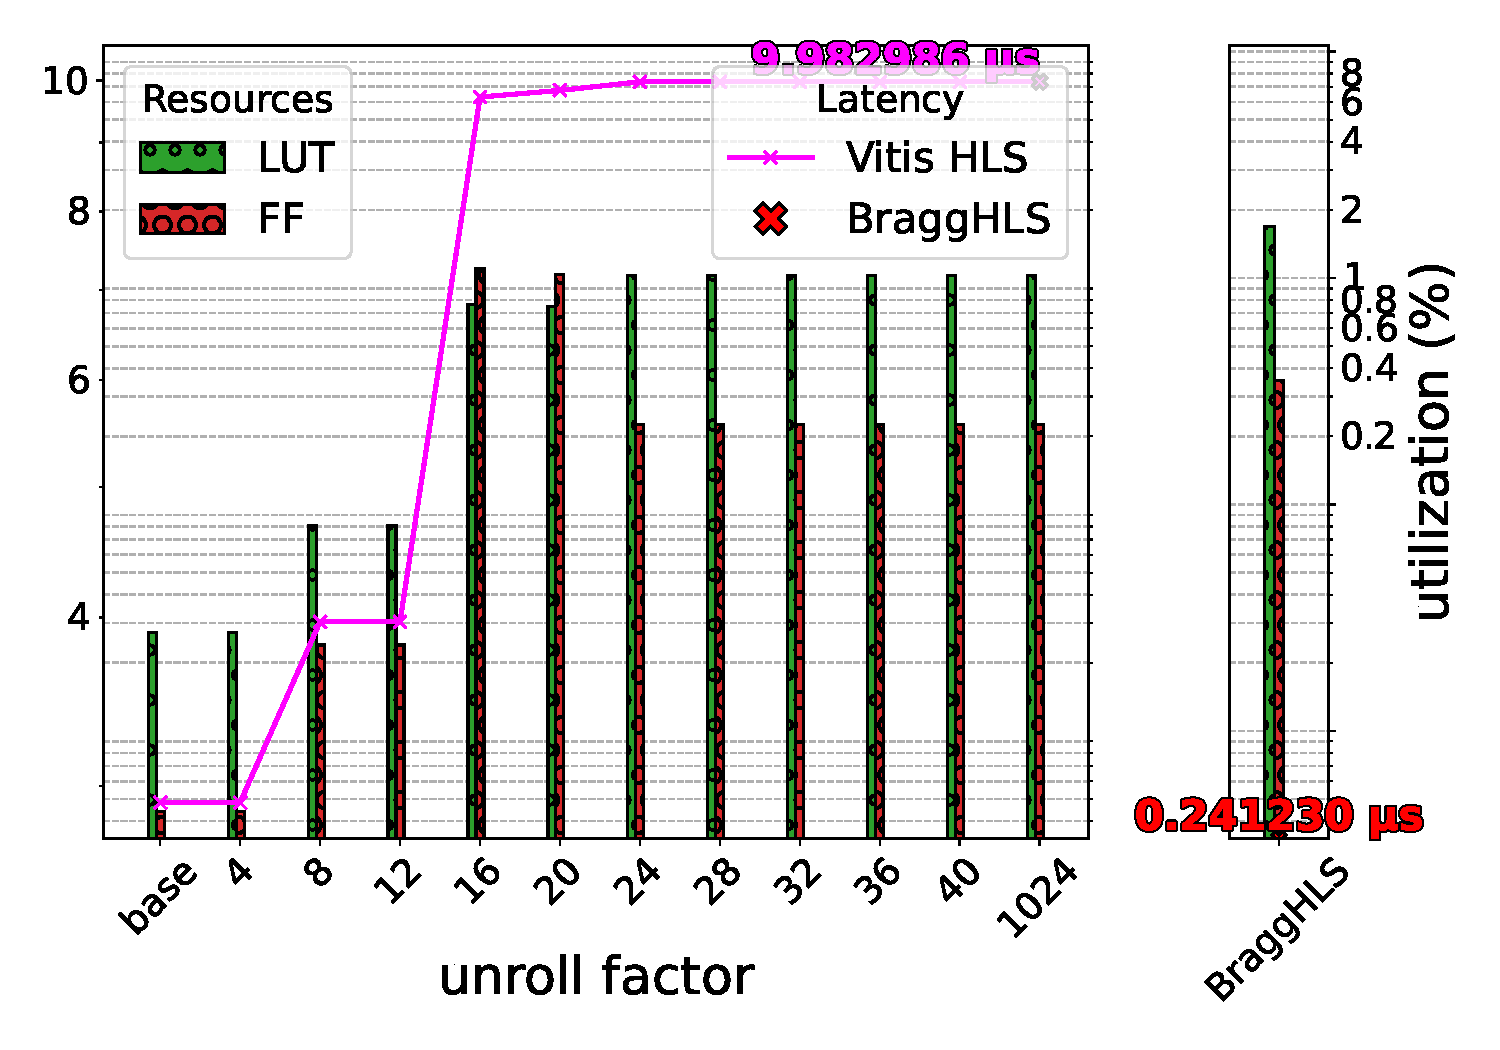
\includegraphics[width=1\columnwidth]{../figures/max_pool_2d}\label{2dlattice-1-2-1-1}}\caption{Resource usage and latency vs. unroll factor of various DNN modules.}
\end{figure*}
\begin{figure*}[tbh]
\centering{}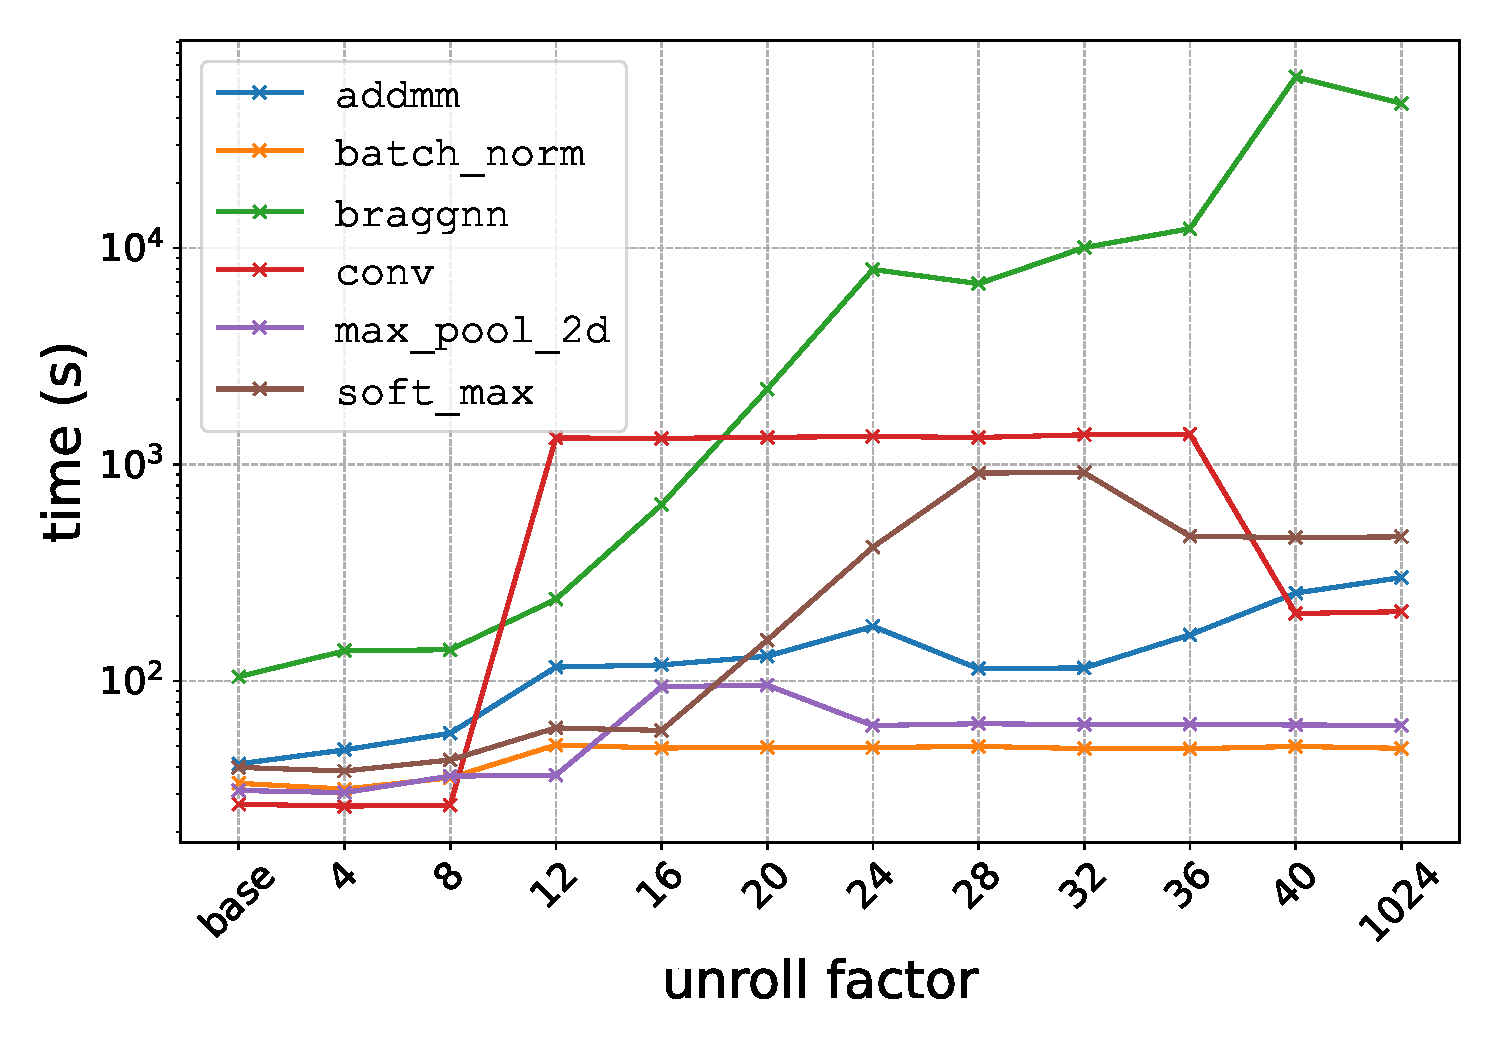
\includegraphics[width=1\columnwidth]{../figures/elapsed_time}\caption{Runtime of Vitis HLS vs. unroll factor.}
\end{figure*}


\subsection{\texttt{BraggNN} case study\label{sec:BraggNN-case-study}}

TODO: put the comparison to both the dataflow pipelined numbers and
the fully unrolled numbers for braggnn here (save the other eval section
for just ops).
\begin{figure}[tbh]
\centering{}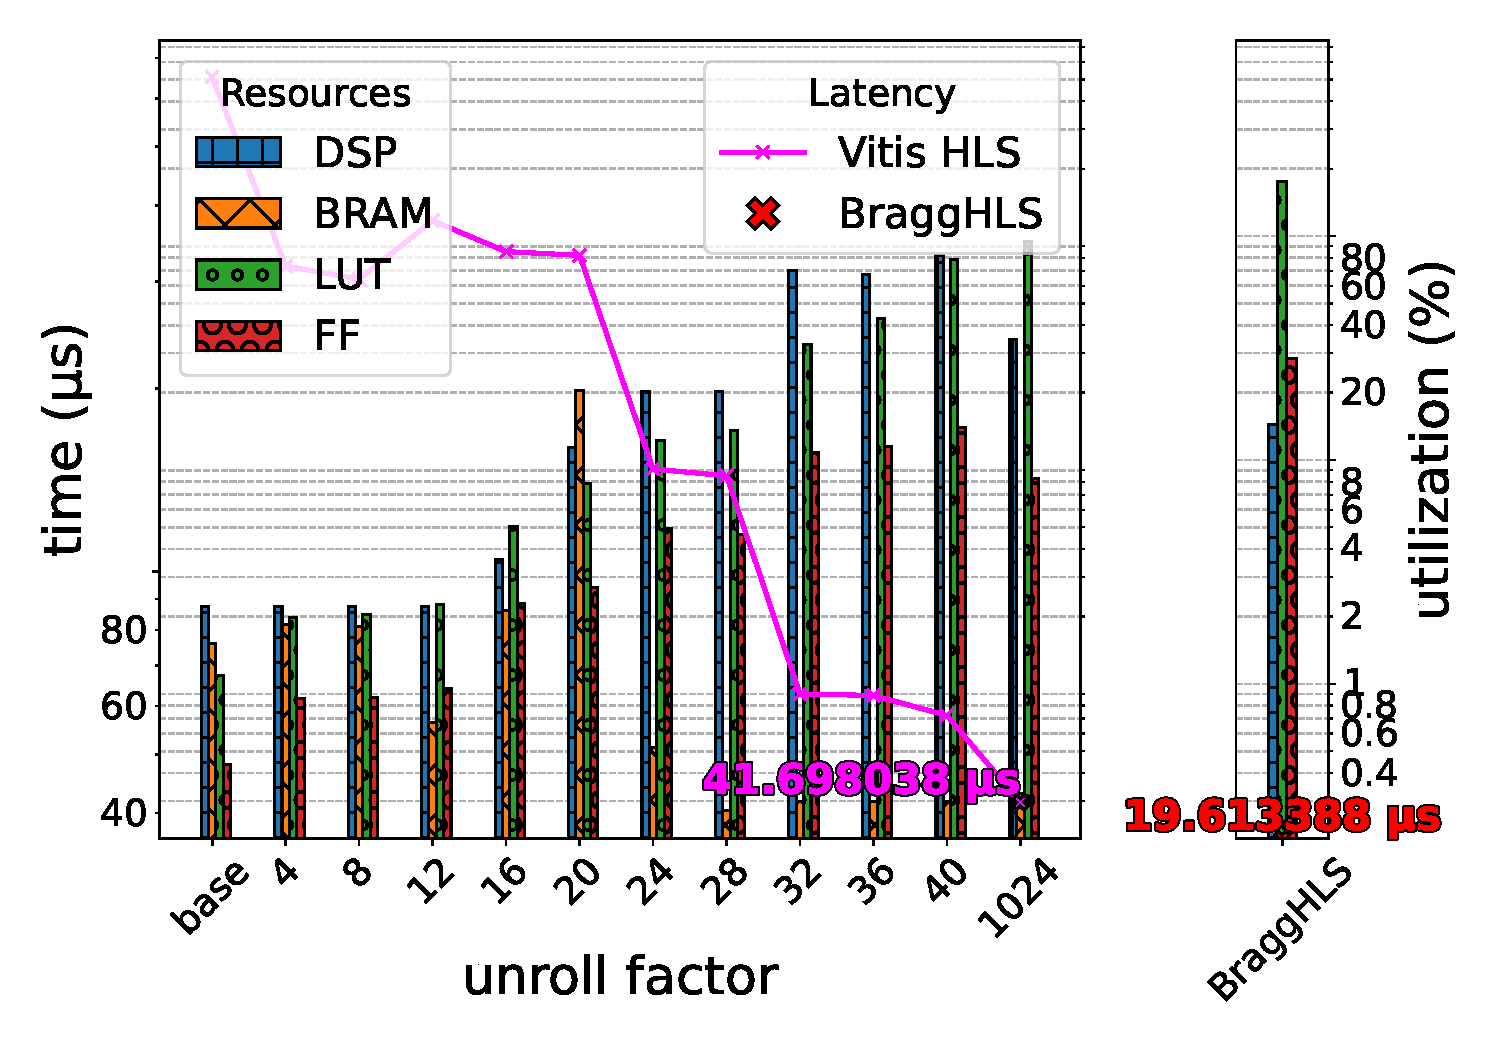
\includegraphics[width=1\columnwidth]{../figures/braggnn}\caption{\texttt{braggnn}}
\end{figure}

High-energy diffraction microscopy techniques can provide non-destructive
characterization for a broad class of single-crystal and polycrystalline
materials. The critical steps in a typical HEDM experiment involve
an analysis to determine precise Bragg diffraction peak characteristics
(and reconstruction of material grain information from the peak characteristics).
Peak characteristics are typically computed by fitting the peaks to
a probability distribution, e.g., Gaussian, Lorentzian, Voigt, or
Pseudo-Voigt. As already mentioned (in Section \ref{sec:Introduction})
the experiments can have collection rates of 80 GB/s. The data rates,
though more modest than those observed at the LHC, combined with the
runtime of the fitting procedure, merit exploring the same low latency
approach in order to enable experimental modalities that depend on
measurement-based feedback (i.e., experiment steering). 
\begin{listing}
\begin{minted}[fontsize={\footnotesize},escapeinside={||},mathescape=true]{python}
BraggNN(
  (cnn_layers_1): Conv2d(|$k \times 16 $|, kernel=3, stride=1)
  (nlb): NLB(
    (theta_layer): Conv2d(|$k \times 16 $|, |$k \times 8 $|, kernel=1, stride=1)
    (phi_layer): Conv2d(|$k \times 16 $|, |$k \times 8 $|, kernel=1, stride=1)
    (g_layer): Conv2d(|$k \times 16 $|, |$k \times 8 $|, kernel=1, stride=1)
    (out_cnn): Conv2d(|$k \times 8 $|, |$k \times 16 $|, kernel=1, stride=1)
    (soft): Softmax()
  )
  (cnn_layers_2): Sequential(
    (0): ReLU()
    (1): Conv2d(|$k \times 16 $|, |$k \times 8 $|, kernel=3, stride=1)
    (2): ReLU()
    (3): Conv2d(|$k \times 8 $|, |$k \times 2 $|, kernel=3, stride=1)
    (4): ReLU()
  )
  (dense_layers): Sequential(
    (0): Linear(in_features=|$k \times 50$|, out_features=|$k \times 16 $|)
    (1): ReLU()
    (2): Linear(in_features=|$k \times 16 $|, out_features=|$k \times 8 $|)
    (3): ReLU()
    (4): Linear(in_features=|$k \times 8 $|, out_features=|$k \times 4 $|)
    (5): ReLU()
    (6): Linear(in_features=|$k \times 4 $|, out_features=2)
    (7): ReLU()
  )
)
\end{minted}
\caption{\texttt{BraggNN} for $k=1,\dots,4$.\label{lis:Single-filter-convolution-3}}
\end{listing}

\texttt{BraggNN} \cite{Liu:fs5198}, a DNN aimed at efficiently characterizing
Bragg diffraction peaks, achieves a batched latency of 22 \textmu s/sample.
This is a large speedup over the classical pseudo-Voigt peak fitting
methods, but still falls far short of the 1 \textmu s/sample target
for handling the 1 MHz sampling rates. In addition, the current implementation
of \texttt{BraggNN}, deployed to either a data-center class GPU such
as a NVIDIA V100, or even a workstation class GPU such as a NVIDIA
RTX 2080Ti, has no practicable means to being deployed at the edge,
i.e., adjacent or proximal to the high energy microscopy equipment.
We applied \texttt{BraggHLS} to the PyTorch representation of \texttt{BraggNN}\emph{
}(see Listing \ref{lis:Single-filter-convolution-3}) and achieve
a RTL implementation which synthesizes to a 1,238 interval design
that places, routes, and meets timing closure for a clock period of
10 ns (for a Xilinx Alveo U280). The design consists of a three stage
pipeline with long stage measuring 480 intervals. Thus, the throughput
of the implementation is 4.8 \textmu s/sample. See Table \ref{tab:Resource-usage-for}
for a summary of the resource usage of the implementation.
\begin{table*}[tbh]
\caption{Resource usage for \texttt{BraggNN} with $k=1$ and $\left(5,3\right)$-precision
FloPoCo \label{tab:Resource-usage-for}}

\begin{centering}
\begin{tabular}{lllllll}
\toprule 
Site Type & SLR0 & SLR1 & SLR2 & SLR0 \% & SLR1 \% & SLR2 \%\tabularnewline
\midrule 
CLB & 5047 & 52648 & 53900 & 9.18 & 97.50 & 99.81\tabularnewline
\midrule 
\quad{}CLBL & 2773 & 28613 & 29227 & 9.47 & 97.72 & 99.82\tabularnewline
\midrule 
\quad{}CLBM & 2274 & 24035 & 24673 & 8.86 & 97.23 & 99.81\tabularnewline
\midrule 
CLB LUTs & 19797 & 263733 & 311794 & 4.50 & 61.05 & 72.17\tabularnewline
\midrule 
\quad{}LUT as Logic & 19797 & 263733 & 311794 & 4.50 & 61.05 & 72.17\tabularnewline
\midrule 
\quad{}\quad{}using O5 output only & 277 & 3944 & 4304 & 0.06 & 0.91 & 1.00\tabularnewline
\midrule 
\quad{}\quad{}using O6 output only & 17176 & 202564 & 266733 & 3.91 & 46.89 & 61.74\tabularnewline
\midrule 
\quad{}\quad{}using O5 and O6 & 2344 & 57225 & 40757 & 0.53 & 13.25 & 9.43\tabularnewline
\midrule 
\quad{}LUT as Memory & 0 & 0 & 0 & 0.00 & 0.00 & 0.00\tabularnewline
\midrule 
\quad{}\quad{}LUT as Distributed RAM & 0 & 0 & 0 & 0.00 & 0.00 & 0.00\tabularnewline
\midrule 
\quad{}\quad{}LUT as Shift Register & 0 & 0 & 0 & 0.00 & 0.00 & 0.00\tabularnewline
\midrule 
CLB Registers & 12527 & 286226 & 339820 & 1.42 & 33.13 & 39.33\tabularnewline
\midrule 
CARRY8 & 244 & 5184 & 5184 & 0.44 & 9.60 & 9.60\tabularnewline
\midrule 
Block RAM Tile & 0 & 0 & 0 & 0.00 & 0.00 & 0.00\tabularnewline
\midrule 
\quad{}\quad{}RAMB36/FIFO & 0 & 0 & 0 & 0.00 & 0.00 & 0.00\tabularnewline
\midrule 
\quad{}\quad{}RAMB18 & 0 & 0 & 0 & 0.00 & 0.00 & 0.00\tabularnewline
\midrule 
URAM & 0 & 0 & 0 & 0.00 & 0.00 & 0.00\tabularnewline
\midrule 
DSPs & 0 & 0 & 0 & 0.00 & 0.00 & 0.00\tabularnewline
\midrule 
Unique Control Sets & 189 & 2641 & 3179 & 0.17 & 2.45 & 2.94\tabularnewline
\bottomrule
\end{tabular}
\par\end{centering}
\bigskip{}

\begin{centering}
\caption{Super long line usage across super logic regions for \texttt{BraggNN}\label{tab:Resource-usage-for-1}}
\par\end{centering}
\centering{}%
\begin{tabular}{lllll}
\toprule 
~ & Used & Fixed & Available & Util \%\tabularnewline
\midrule 
SLR2 $\leftrightarrow$ SLR1 & 21366 & ~ & 23040 & 92.73\tabularnewline
\midrule 
SLR1 $\rightarrow$ SLR2 & 2 & ~ & ~ & < 0.01\tabularnewline
\midrule 
SLR2 $\rightarrow$ SLR1 & 21364 & ~ & ~ & 92.73\tabularnewline
\midrule 
SLR1 $\leftrightarrow$ SLR0 & 3904 & ~ & 23040 & 16.94\tabularnewline
\midrule 
SLR0 $\rightarrow$ SLR1 & 2 & ~ & ~ & < 0.01\tabularnewline
\midrule 
SLR1 $\rightarrow$ SLR0 & 3902 & ~ & ~ & 16.94\tabularnewline
\midrule 
Total SLLs Used & 25270 & ~ & ~ & ~\tabularnewline
\bottomrule
\end{tabular}
\end{table*}

The most challenging aspect of implementing \texttt{BraggNN} was minimizing
latency while satisfying compute resource constraints (LUTs, DSPs,
BRAMs) and meeting routing ``closure'', i.e., not exceeding available
routing resources and avoiding congestion. Two design choices made
for the purposes of reducing resource consumption was reducing the
precision used for the floating-point operations. We reduced the precision
from IEEE half precision (5 bits for the exponent and 11 bits for
the mantissa) to FloPoCo $\left(5,4\right)$-precision (5 bits for
the exponent and 4 bits for the mantissa). This was justified by an
examination of the distribution of the weights of the fully trained
\texttt{BraggNN} (see figure \ref{fig:BraggHLS-framework-overview.-1}).
\begin{figure}[tbh]
\centering{}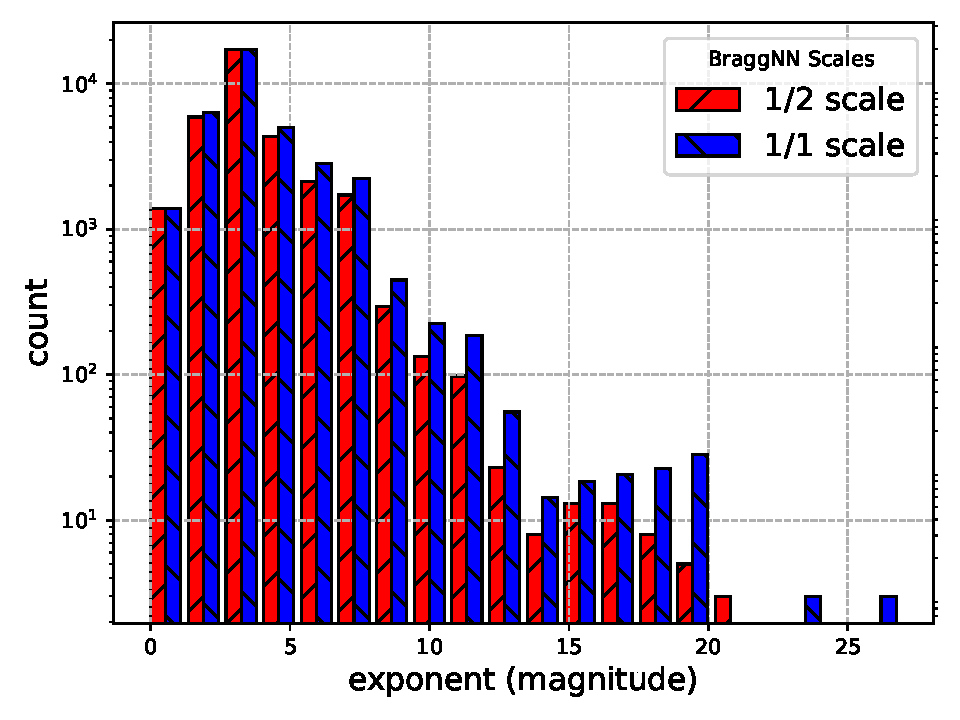
\includegraphics[width=1\columnwidth]{../figures/exp_hist}\caption{\texttt{BraggHLS} weights exponent distribution.\label{fig:BraggHLS-framework-overview.-1}}
\end{figure}
 Reducing the precision enabled us to eliminate BRAMs from the design
as well, since, at the lower precision, all weights could be represented
as registered constants. The reduced precision also drives the Vivado
synthesizer to infer implementations of the floating-point operations
that make no use of DSPs; this was not intentional but seemingly cannot
be altereted. Most likely this is due to the fact that DSP48 hardware
block includes a 18-bit by 25-bit signed multiplier and a 48-bit adder
\cite{guideultrascale}, neither of which neatly divide the bit width
of FloPoCo $\left(5,4\right)$-precision cores\footnote{The actual bit width for FloPoCo $\left(5,4\right)$-precision is
12 bits: 1 extra bit is needed for the sign and 2 bits are needed
for FloPoCo's handling of exceptional conditions.}.

Achieving routing closure was very difficult due to the nature of
the Xilinx's UltraScale architecture, of which the Alveo U280 is an
instance. The UltraScale architecture achieves its scale through ``Stacked
Silicon Interconnect'' (SSI) technology \cite{leibson2013xilinx},
which amounts to multiple distinct FPGA dies, called Super Logic Regions
(SLRs), on the same chip, connected by interposers. Adjacent SLRs
communicate with each other using a limited set of Super Long Lines
(SLLs). These SLLs determine the maximum bus width that span two SLRs.
On the Alveo U280 there are exactly 23,040 SLLs available between
adjacent SLRs and at $\left(5,4\right)$-precision \texttt{BraggNN}
needs 23,328 SLLs between SLR2 and SLR1\footnote{We route the output of \texttt{cnn\_layers\_1} ($1\times16\times9\times9\times12$
wires) as well as the output of $\texttt{soft(theta\_layer}\times\texttt{phi\_layer)}\times\texttt{g\_layer}$
($1\times8\times9\times9\times12$ wires) from SLR2 to SLR1.}. Thus, we further reduce the precision to $\left(5,3\right)$. Finally,
since multiple dies constitute independent clock domains, the SLLs
that cross SLRS are sensitive hold time violations due to the higher
multi-die variability \cite{rapidwright}. This multi-die variability
leads to high congestion if not addressed. Thus, routing across them
needs to handled manually using placement and routing constraints
for logic in each SLR and the addition of so-called ``launch'' and
``latch'' registers in each SLR. See figure \ref{fig:BraggHLS-framework-overview.-2}
for an illustration on the effect of using launch and latch registers
as well as placement and routing constraints.
\begin{figure*}[tbh]
\centering{}\subfloat[\texttt{BraggNN} fails to achieve routing closure without placement
and routing constraints and launch and latch registers.\label{fig:BraggHLS-framework-overview.-2-1}]{\centering{}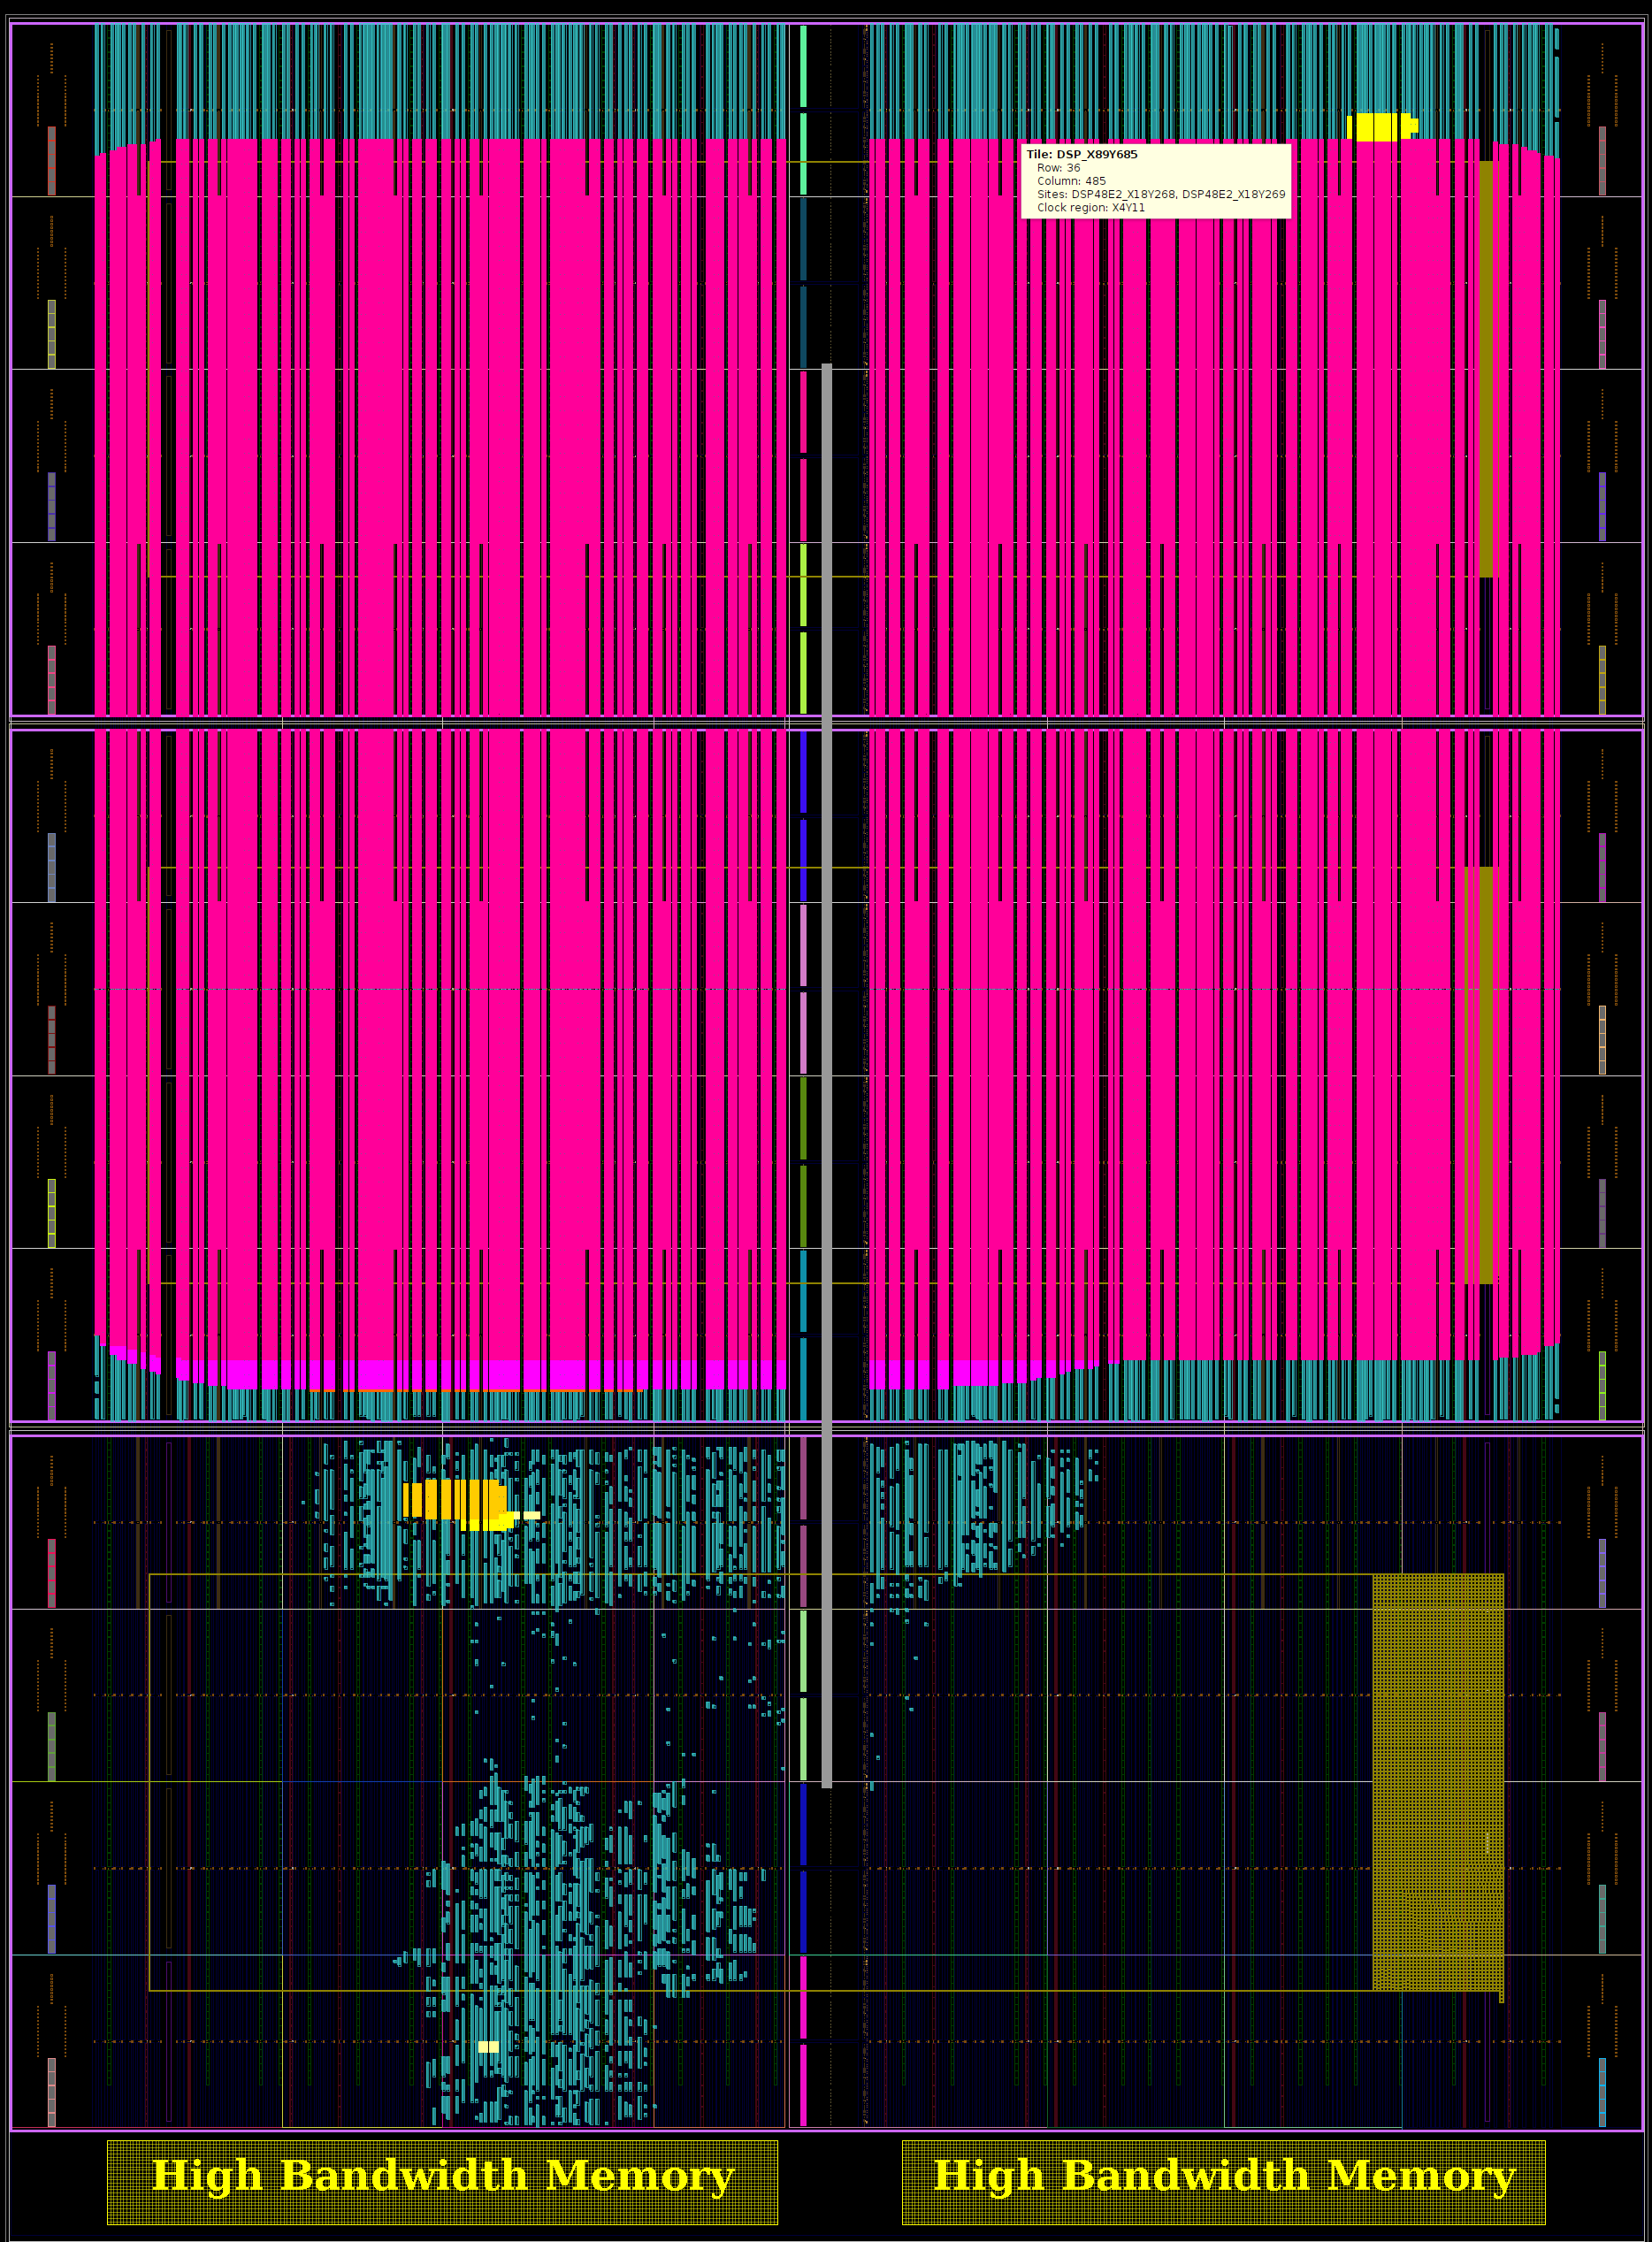
\includegraphics[width=1\columnwidth]{nopblocks}}\hfill{}\subfloat[\texttt{BraggNN} achieves routing closure with use of per SLR placement
and routing constraints (\texttt{pblock\_1}, \texttt{pblock\_2}, \texttt{pblock\_3})
and launch and latch registers (not highlighted).\label{fig:BraggHLS-framework-overview.-2-1-1}]{\centering{}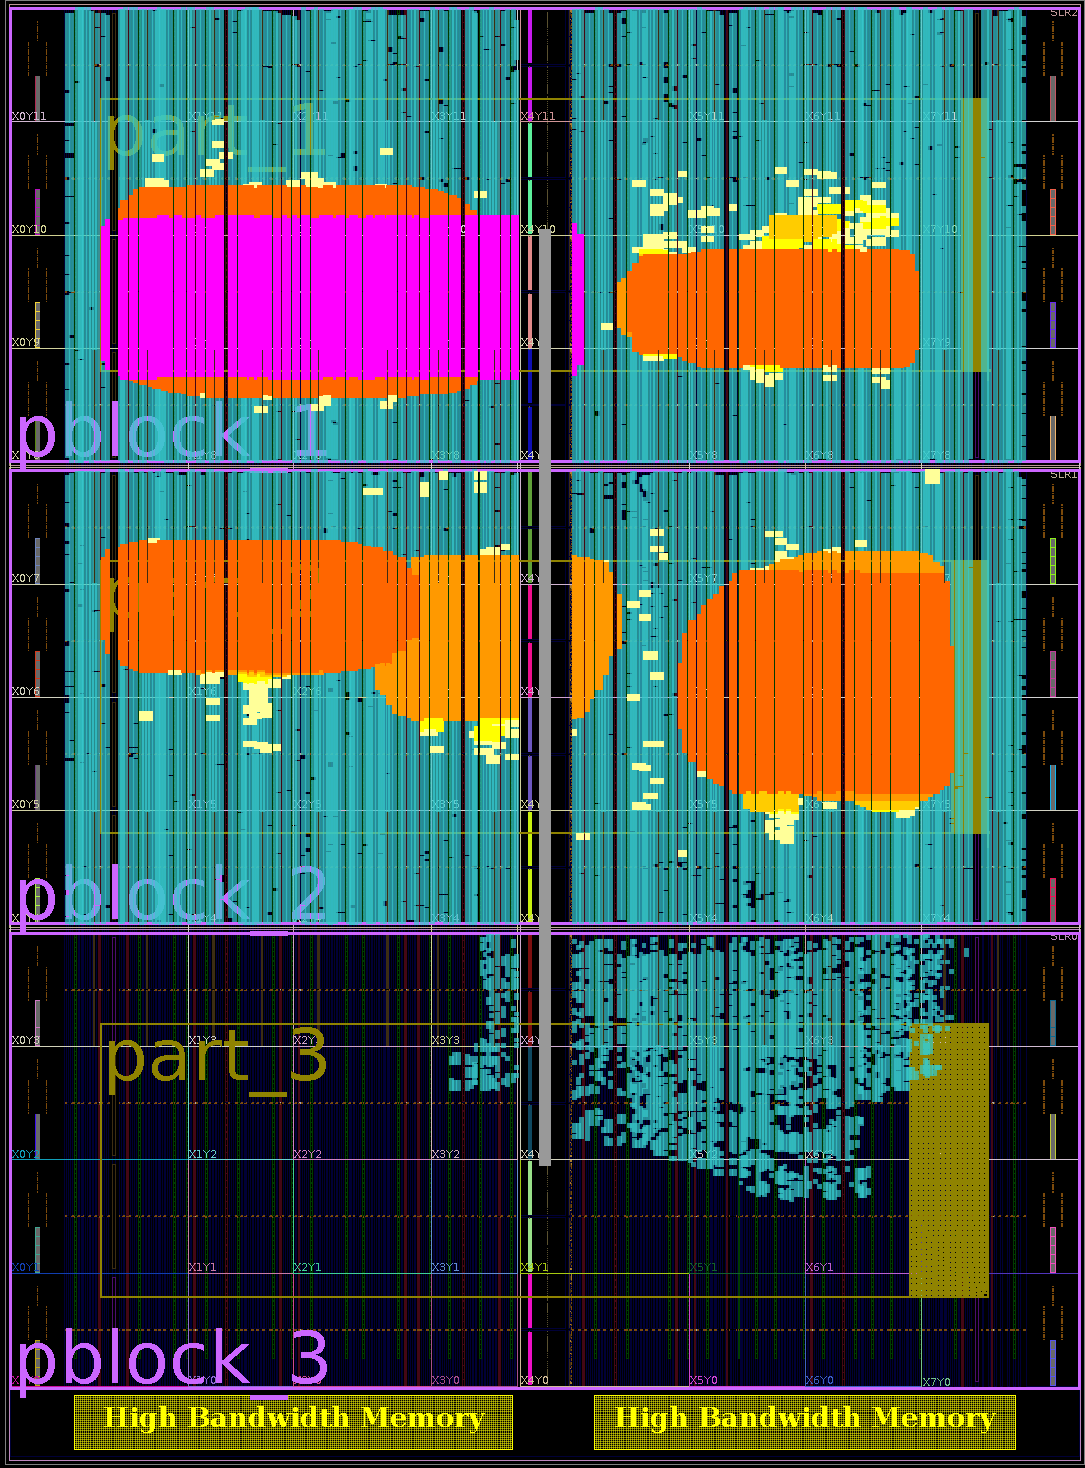
\includegraphics[width=1\columnwidth]{withpblocks}}\caption{Congestion maps for \texttt{BraggNN} on a Xilinx Alveo U280. \textcolor{magenta}{Magenta}
indicates area of high congestion.\label{fig:BraggHLS-framework-overview.-2}}
\end{figure*}


\section{Conclusion\label{sec:Conclusion}}

287 + 471 + 480

\bibliographystyle{IEEEtran}
\bibliography{ref}

\end{document}
